%This file is the main file where the final document is generated

\documentclass{these-ubl} 
\usepackage{bibunits}
\geometry{vmargin=4.0cm}

%Pour diff\'{e}rentes universit\'{e}s il faurdra modifier ce d\'{e}but de document
%For different universities modify the beginning of this document to adapt the logos (logo)
\geometry{vmargin=4.0cm}
\logoecoledoc{./Couverture-these/MathSTIC/logo-mathSTIC} %logo ecole doctorale
\logoetablissement{./Couverture-these/MathSTIC/logo-etablissements/logoUR1}%logo etablissement (ici Rennes 1) 
\vspace{2.5cm}
%Indiquer l'\'{e}tablissement de d\'{e}livrance du diplome
%Provide the name of the institution that delivers the diploma, 
\unite{L'UNIVERSIT\'{E} DE RENNES 1}
%Si la th\`{e}se est en co-tutelle ou en d\'{e}livrance conjointe, mettre le logo des 2 \'{e}tablissements 
%in the case of "co-tutelle" provide both names (logos)
\ubl{Comue Université Bretagne Loire}
%Indiquer le num\'{e}ro d’accr\'{e}ditation de l’\'{e}cole doctorale de r\'{e}f\'{e}rence pour la th\`{e}se 
%indicate the certification number of l'ecole doctorale
\ecoledoc{\'{E}cole Doctorale N° 601}
%Indiquer le nom de l’\'{e}cole doctorale de r\'{e}f\'{e}rence pour la th\`{e}se 
%Indicate the name of l'ecole doctorale
\nomecole{Math\'{e}matiques et Sciences et Technologies \\ de l'Information et de la Communication}
%Inscrivez ici votre sp\'{e}cialit\'{e} (voir liste des sp\'{e}cialit\'{e}s sur le site de votre \'{e}cole doctorale)
%Indicate the domain (see list of domains in your ecole doctorale)
\spec{Sp\'{e}cialit\'{e} : \textit{(voir liste des sp\'{e}cialit\'{e}s)}}
\usepackage{eso-pic}


\begin{document}

% PDF document Tags
\hypersetup{
    pdftitle={title},    % title
    pdfauthor={author},     % author
    pdfsubject={Subject},   % subject of the document
    pdfcreator={creator},   % creator of the document
    pdfproducer={producer}, % producer of the document
    pdfkeywords={Green Networking} {Mobile Cloud} {Network Coding} {Energy} % 
}

% La page de garde est en français
% The front cover is in French
\selectlanguage{french}

%background image of the front cover
\AddToShipoutPicture*{%
    \put(0,0){%
    \parbox[b][42.5cm]{\paperwidth}{%
        \vfill
        
\includegraphics[width=\paperwidth,keepaspectratio]{./Couverture-these/MathSTIC/image-fond-MATHSTIC-gardeO.png}% image de fond UR1
        \vfill
}}}
%Attention : le pr\'{e}nom doit être en minuscules (Jean) et le NOM en majuscules (BRITTEF) 
%Attention : the first name in small letters and the name in Capital letters 
\author{« Pr\'{e}nom NOM »}
% Donner le titre complet de la th\`{e}se, \'{e}ventuellement le sous titre, si n\'{e}cessaire sur plusieurs lignes 
%Give the complete title of the thesis, if necessary on several lines
\title{« Titre de la th\`{e}se »}
\lesoustitre{« Sous-titre de la th\`{e}se »}
%Indiquer la date et le lieu de soutenance de la th\`{e}se 
%indicates the date and the place of the defense 
\date{« date »}
\lieu{« Lieu »}
%Indiquer le nom du (ou des) laboratoire (s) dans le(s)quel(s) le travail de th\`{e}se a \'{e}t\'{e} effectu\'{e}, indiquer aussi si souhait\'{e} le nom de la (les) facult\'{e}(s) (UFR, \'{e}cole(s), Institut(s), Centre(s)...), son (leurs) adresse(s)... 
%Indicates the name (or names) of research laboratories where the work has been done as well as (if desired) the names of faculties (UFR, Schools, institution...
\uniterecherche{Unit\'{e} de recherche : }
%Indiquer le Numero de th\`{e}se, si cela est opportun, ou faire disparaitre cet item de la couverture 
%Indicate the number of the thesis if there is one.
\numthese{Th\`{e}se N° :  }
%Indiquer le Pr\'{e}nom en minuscules et le Nom en majuscules, le titre de la personne et l’\'{e}tablissement dans lequel il effectue sa recherche  
%Indicates the first name on small letters and the Names on capital letters, the person's title and the institution where he/she belongs to.
%Exemples :  Examples :
%%%- Professeur, Universit\'{e} d’Angers 
%%%- Chercheur, CNRS, \'{e}cole Centrale de Nantes 
%%%-  Professeur d’universit\'{e} – Praticien Hospitalier, Universit\'{e} Paris V  
%%%-  Maitre de conf\'{e}rences, Oniris 
%%%- Charg\'{e} de recherche, INSERM, HDR, Universit\'{e} de Tours  
 %S’il n’y a pas de co-direction, faire disparaitre cet item de la couverture  
 %In there is no co-director, remove the item from the cover


\jury{
{\normalsize \textbf{Rapporteurs avant soutenance :}}\\ \newline
\footnotesize
\begin{tabular}{@{}ll}
Pr\'{e}nom Nom & Fonction et \'{e}tablissement d'exercice \\
Pr\'{e}nom Nom & Fonction et \'{e}tablissement d'exercice \\
Pr\'{e}nom Nom & Fonction et \'{e}tablissement d'exercice \\
\end{tabular}

\vspace{\baselineskip}
{\normalsize \textbf{Composition du Jury :}}\\
{\fontsize{9.5}{11}\selectfont {\textcolor{red}{\textit{Attention, en cas d’absence d’un des membres du Jury le jour de la soutenance, la composition du jury doit être revue pour s’assurer qu’elle est conforme et devra être répercutée sur la couverture de thèse}}}}\\ \newline
\footnotesize
\begin{tabular}{@{}lll}

Pr\'{e}sident :        & Pr\'{e}nom Nom & Fonction et \'{e}tablissement d'exercice \textit{(à préciser après la soutenance)} \\
Examinateurs :         & Pr\'{e}nom Nom & Fonction et \'{e}tablissement d'exercice \\
                       & Pr\'{e}nom Nom & Fonction et \'{e}tablissement d'exercice \\
                       & Pr\'{e}nom Nom & Fonction et \'{e}tablissement d'exercice \\
                       & Pr\'{e}nom Nom & Fonction et \'{e}tablissement d'exercice \\
Dir. de th\`{e}se :    & Pr\'{e}nom Nom & Fonction et \'{e}tablissement d'exercice \\
Co-dir. de th\`{e}se : & Pr\'{e}nom Nom & Fonction et \'{e}tablissement d'exercice \textit{(si pertinent)} \\
\end{tabular}

\vspace{\baselineskip}
{\normalsize \textbf{Invit\'{e}(s) :}}\\
\footnotesize
\begin{tabular}{@{}ll}
Pr\'{e}nom Nom & Fonction et \'{e}tablissement d'exercice \\
\end{tabular}
}


\maketitle
 % page de garde UR1

% Select the content language following this line
\selectlanguage{english}

%input acknowledgement chapter 
\clearemptydoublepage
\chapter*{Acknowledgement}

Je tiens à remercier  \\
I would like to thank. my parents..\\
J'adresse également toute ma reconnaissance à .... \\
....


%Inut resume en Francais
\clearemptydoublepage
\begin{bibunit}[IEEEtran.bst]

\chapter*{Résumé en français}
Cette thèse explore comment les avancées en apprentissage profond peuvent aider à l'analyse des mesures satellitaires de la hauteur de surface de la mer (SSH). Les altimètres actuels fournissent des données échantillonnées de manière irrégulière avec un faible couverture spatiale, limitant ainsi l'observation de processus prenant places aux petites échelles. Repousser cette limite améliorerait notre connaissance des dynamique de la surface de l'océan ainsi que nos capacités de surveillance du climat. De nouvelles opportunités pour renforcer nos capacités d'observation ont émergé avec le déploiement du capteur KaRIn lors de la mission SWOT.

Ces dernières années, les approches d'apprentissage ont démontré des capacités remarquables en vision par ordinateur et en traitement du langage naturel. Contrairement à de telles tâches, les problèmes d'observations océaniques peuvent impliquer de forts a priori physiques ainsi que peu de données annotées. Ce travail aborde les considérations spécifiques de l'application de l'apprentissage profond aux données altimétriques en trois parties.

Premièrement, à travers l'étalonnage du capteur KaRIn, nous démontrons comment des connaissances spécifiques du domaine peuvent être intégrées dans les cadres d'apprentissage profond. Nous montrons spécifiquement comment le budget d'erreur spectral de la mission SWOT peut informer la conception d'architectures neuronales.

Deuxièmement, nous abordons la rareté des données de vérité terrain lors de la conception de méthodes neuronales d'interpolation de données altimétriques. Nous illustrons comment les simulations de modèles océaniques et de systèmes d'observation peuvent surmonter ce défi en fournissant des environnements d'entraînement supervisés qui se généralisent aux données réelles.

Enfin, notre troisième contribution traite des défis rencontrés pour combler le fossé entre les communautés "océan" et "apprentissage profond". Une collaboration efficace nécessite que des experts de l'océan définissent les défis d'intérêt ainsi que la méthode adéquate d'évaluer les solutions. Le praticien en apprentissage automatique nécessite de son côté les outils nécessaires pour accéder et manipuler les différentes données pertinentes.  Nous décrivons comment nous avons abordé ces aspects lors du développement du projet OceanBench.

% \section*{Motivations}

% \section*{Objectifs}

% \section*{Contributions}

% \section*{Contenu du manuscrit}

% In this manuscript I'd like to cite \cite{remo1,remo2}.

% \putbib[./Resume-Francais/Res-Biblio.bib]
\end{bibunit}

%This command will generate the front cover
\clearemptydoublepage
\frontmatter 
\renewcommand{\contentsname}{Table of Contents}
\setcounter{tocdepth}{5}
\tableofcontents %sommaire %table of content

\clearemptydoublepage
\chapter*{List of acronyms}
\addcontentsline{toc}{chapter}{List of acronyms}
\chaptermark{List of acronyms}


\begin{tabular}{ll}
4DVAR & Four Dimensional Variational Data Assimilation\\
3DVAR & Three Dimensional Variational Data Assimilation\\
BFN & Back-and-Forth Nudging\\
CV  & Computer Vision\\
DL & Deep Learning \\
DUACS & Data Unification and Altimeter Combination System\\
DYMOST & Dynamic Interpolation Ocean Science Topography\\
KaRIn & Ka-band Radar Interferometer\\
KF & Kalman Filter \\
L4 & Level 4\\
MDT & Mean Dynamic Topography\\
MIOST & Multiscale Interpolation Ocean Science Topography\\
ML & Machine Learning\\
NEMO & Nucleus for European Modelling of the Ocean\\
NLP &  Natural Language Processing\\
nRMSE & normalized Root Mean Squared Error\\
OSE  & Observing System Experiment\\
OSSE  & Observing System Simulation Experiment\\
PSD & Power Spectrum Density\\
QG & Quasi-Geostrophic\\
RMSE & Root Mean Squared Error\\
SLA & Sea Level Anomaly\\
SSH & Sea Surface Height\\
SWOT &  Surface Water Ocean Topography \\


% AAM & Active Appearance Models \\
% ANN & Artificial Neural Networks \\
% APSS & Association of the Psychophysiological Study of Sleep \\ 
% AR & Auto Regressive \\
% AS & Active Sleep \\
% AU & Action Unit \\
% AUC & Area Under Curve \\
% B\&W & Black and White \\
% CCHS & Congenital Central Hypoventilation Syndrome \\
% CNN & Convolution Neural Networks \\
% CNS & Central Nervous System \\
% CP & Cerebral Palsy \\
% CU & Cry Unit \\
% CWT & Continuous Wavelet Transform \\
% D & Drowsiness \\
% DAN & Douleur Aig{\"u}e du Nouveau-n{\'e} \\
% DCT & Discrete Cosinus Transform \\
%
\end{tabular}
%
% \begin{tabular}{ll}
% KLT & Kanade-Lucas-Tomasi \\
% KNN & K-Nearest Neighbors \\
% LDA & Linear Discriminant Analysis \\
% LOOCV & Leave-one-out cross-validation \\
% LPCCs & Linear Prediction Cepstral Coefficients \\
% LR & Logistic Regression \\
% LTAS & Long Time Average Spectrum \\
% MFCCs & Mel Frequency Cepstral Coefficients \\
% MLE & Maximum Likelihood Estimation \\
% MLP & Multi-Layer Perceptron \\
% NBAS & Neonatal Behavioral Assessment Scale \\
% NFCS & Neonatal Facial Coding System \\
% NICU & Neonatal Intensive Care Units\\
% NIDCAP & Newborn Individualized Developmental Care and Assessment Program  \\
% NIR & Near-InfraRed \\
% NLEO & Non Linear Energy Operator \\
% NUC & Next Unit of Computing \\
% OSA & Obstructive Sleep Apnea \\
% PCA & Principal Component Analysis \\
% PMA & PostMenstrual Age \\
%
%
% \end{tabular}
%



\listoffigures
\addcontentsline{toc}{chapter}{List of figures}

\listoftables
\addcontentsline{toc}{chapter}{List of tables} 

\clearemptydoublepage
\begin{bibunit}[IEEEtran.bst]

\chapter*{Introduction}
\addcontentsline{toc}{chapter}{Introduction}
\chaptermark{Introduction}


\section*{Motivation}
\addcontentsline{toc}{section}{Motivation}

Understanding and anticipating the ramifications of climate change represents a pressing challenge of our era. Enhancing our knowledge of Earth's systems is a key factor in confronting this challenge. Given that the primary source of factual information about the Earth system is observational data, improving our ability to exploit this data could lead to better monitoring and understanding of our planet. Concurrently, recent advancements in deep learning provide robust tools that continually push performance boundaries across a myriad of tasks. This situation raises an intriguing question: Can deep learning assist in extracting meaningful insights from Earth observations?

Observing ocean surface dynamics through satellite altimetry offers a compelling case study. Currently, operational products do not resolve processes below 150 km, which are essential for climate monitoring. This situation underscores a significant gap in our observational capabilities. The recent deployment of a novel sensor during the SWOT satellite mission provides numerous opportunities to address this gap. This new sensor introduces unprecedented calibration challenges due to previously unseen errors, but it also promises to enhance the reconstruction of Sea Surface Height (SSH) maps.

Despite the significant potential of deep learning, two critical factors seem to determine progress in a specific domain. The first factor is quality and availability of data, indeed the creation of large, curated datasets, like ImageNet in computer vision or ThePile in natural language processing have shown to dramatically expedite the development of novel approaches. The second factor is the design of architectural patterns that are particularly suited to given problem, leading to performance breakthroughs. Examples of these include convolution techniques in computer vision, attention mechanisms in natural language processing, and U-Net architectures for hierarchical data. These two facets — comprehensive, well-curated datasets and efficient architectural patterns — can greatly advance the field, propelling research and application development in exciting directions.

The transdisciplinary nature of this work also introduces unique challenges. The intricacies of ocean observation data and the criteria for precisely evaluating the estimation of geophysical quantities can represent a considerable barrier for ML scientists. Similarly, the logistical aspects and accumulated best practices required to successfully train and utilize a neural network can deter domain experts from leveraging the latest advancements.

The first chapter of this thesis will present a generic problem formulation that aligns domain expert methods and deep learning approaches within a unified ontology. This will lay a solid foundation for understanding how these two domains provide complementary perspectives on a problem and can potentially be integrated. Additionally, this chapter will serve as a review of the state-of-the-art in this research area.

The next two chapters of this dissertation consider two use cases that correspond to different stages of altimetry data analysis while shedding light on various deep learning challenges.

The second chapter delves into the calibration of the SWOT KaRIn data, examining how to separate the SSH from error signals. From a learning standpoint, this chapter showcases a method for integrating the a priori knowledge we have about error signals into the architectural design of a neural-based method.

The third chapter emphasizes the challenges of training neural mapping schemes on observational data due to the uncertainty about the true state of the ocean. It focuses on the task of interpolating SSH fields with a high rate of missing data. The chapter further demonstrates that current numerical simulations of the ocean permit the training of a neural data assimilation scheme that generalizes effectively to real data.

The subsequent two chapters document our efforts to facilitate the collaboration between the ML and ocean observation communities. Chapter four introduces a comprehensive toolbox for designing and evaluating ML problems related to altimetry mapping. Chapter 5 presents a didactic and modular implementation of the 4DVarNet deep learning algorithm, which has seen use in a variety of publications related to ocean observation data.


% Understanding and anticipating the implications of climate change is a pressing challenge of our era, and improving our knowledge of Earth's systems is a critical factor in meeting this challenge. Given that factual information about the state of the Earth system is derived from observational data, the recent advancements in deep learning provide potent tools for enhancing our knowledge, pushing performance boundaries across an expanding range of tasks. This raises an intriguing question: Can deep learning assist in extracting meaningful knowledge from Earth observations?
%
%
% The first source of challenge we can encounter comes from the 
% Observing ocean surface dynamics through satellite altimetry provides an engaging case study. Currently, operational products do not resolve processes below 150 km, which play a pivotal role in climate monitoring. This situation reveals a significant gap in our observational capabilities. The recent deployment of a novel sensor during the SWOT satellite mission presents multiple opportunities to bridge this gap. This new sensor brings unprecedented challenges for calibration due to previously unseen errors and promises the prospect of improving the reconstruction of Sea Surface Height (SSH) maps.
%
%
% Deep learning, while offering significant advantages, also presents certain challenges. Two crucial factors appear to be determinants for progress in a specific domain through deep learning. First is the creation of large, curated datasets, such as ImageNet or The Pile, which can dramatically speed up the development of novel approaches. Second, the discovery of architectural patterns that are well-suited for a specific domain can trigger performance leaps. Examples include convolution techniques in computer vision, attention mechanisms in natural language processing, and U-Net architectures for hierarchical data. These two aspects — well-curated datasets and effective architectural patterns — can fundamentally advance the field, propelling research and application development in novel directions.
%
%   The transdisciplinary aspect of this work also poses unique challenges. The specificities of ocean observation data and the criteria for accurately evaluating the estimation of geophysical quantities can pose a substantial barrier of entry for ML scientists. Similarly, the logistics and accumulated tools and tricks necessary to successfully train and use a neural network can be a hindrance for domain experts wishing to leverage the latest advancements.
%
% The first two chapters of this dissertation look at two use cases that point to different stages of altimetry data analysis while highlighting on different deep learning challenges.
%
% The first chapter focuses on the calibration of the SWOT KaRIn data, and how we can separate the SSH from error signals. From a learning standpoint, this chapter demonstrates a method for incorporating the a priori knowledge we have about the error signals into the architectural design of a neural-based method.
%
% The second chapter highlights the challenges of training neural mapping schemes on observational data due to the lack of knowledge about the true state of the ocean. It focuses on the interpolation taks of SSH fields with a high rate of missing data. It further demonstrates that current numerical simulations of the ocean allow for training a neural data assimilation scheme that generalizes well on real data.
%
% The subsequent two chapters present our efforts to strengthen the bridge between the ML and ocean observation community. Chapter 3 introduces a comprehensive toolbox for designing and evaluating ML problems related to altimetry mapping. In chapter 4, we present a pedagogical and modular implementation of the 4DVarNet algorithm, which has been utilized in a variety of publications related to ocean observation data.
%
%
\section*{Tasks}
\addcontentsline{toc}{section}{Tasks}
  Most tasks can formulated as finding a mapping $f$ from available data $y$ to a quantity of interest $u$

\section*{Methodology}
\addcontentsline{toc}{section}{Methodology}



% Understanding and anticipating the implications of climate change is a critical challenge for our time, and improvements in our knowledge of the Earth's systems are one of the most impactful ways we can meet this challenge. Moreover, given that factual informations we have on the earth system state comes from observation data and that recent advances in deep learning offer us powerful tools to enhance our knowledge, pushing the performance boundaries across a growing range of tasks. This raises the question: can deep learning assist in extracting knowledge from earth observations ?
%
% Observation of ocean surface dynamics through satellite altimetry serves as an interesting case study. Presently, operational products do not resolve processes below 150 km which play a key role in climate monitoring, indicating a significant gap in our observational capabilities. And multiple opportunities arise to reduce this gap with recent deployment of a novel sensor during the SWOT satellite mission. This new sensor brings novel need for calibration of previously unseen errors and opens perspectives of improving the reconstruction of SSH maps.
%
%  Two wings are needed to make a machine learning model fly: the optimization and the generalization. Indeed training a machine learning model consist in searching a parameter space (i.e optimization) to find a model configuration that will perform well on unseen data (generalization). Dataset, training objective and optimization procedure will intervene in the parameter search whereas informed decision on the architecture will determine if the trained model behaves well outside the training context.
%
%correlate with  in deep learning One may see deep learning as generic tools, however we can note how advances i significant advances were made when architectural choice 
% To make a machine learning model perform effectively, both optimization and generalization are vital. Training a machine learning model involves searching a parameter space (i.e., optimization) to find a model configuration that will perform well on unseen data (generalization). The dataset, training objective, and optimization procedure participate in the parameter search, while informed decisions on the architecture determine if the trained model behaves appropriately outside the training context. When applying learning-based methods to a new applicative domain, the choice of data and decision about the architecture should be made in accord with the domain requirements. 


% The transdisciplinary aspect of this work also brings its share of challenges, indeed the specificities  ocean observation data and the criteria for correctly evaluating the estimation of geophysical quantities can be a significant barrier of entry for ML scientist.
%  Similarly the logistics and accumulated tools and tricks necessary to successfully train and use a neural network can be a hindrance for domain experts to take advantages of the latest advances made.
%
% This first two parts look at two use cases that point to different stages of an observation data analysis and that tackle different aspects of the learning challenges.
%
% The first chapter will focus on the beginning of the observing system chain which is the calibration of the SWOT KaRIn data and how we can separate the SSH from error signals. This example showcases a way of incorporating the a priori knowledge we have about the error signals into the architectural design of a neural based method.
%
% The second part will focus on the processing of calibrated data and how to interpolate SSH fields with high rate of missing data. This section highlight the challenges of training neural mapping schemes on observation data by lack of knowledge of the true ocean state and demonstrate that current numerical simulations of the ocean allow for training a neural data assimilation scheme that generalizes well on real data.
%
% The next two chapters present our effort in reinforcing the brigde between the ML and ocean observation community by presenting in chapter 3 a comprehensive tooolbox for designing and evaluating ML problems related to altimetry mapping. In chapter 4 we present a pedagogical and modular implementation of the 4DVarNet algorithm which has been used in a variety of publication related with ocean observation data. 
%
% Welcoming applied ml researchers to altimetry mapping
% Sharing generic neural data assimilation framework
% Sensor calibration inductive biases
% Blind optimization of mapping algorithm
%
% The application of deep learning to satellite altimetry poses its own challenges, the first one of which is to formulate a learning problem that is relevant for domain expert through data and evaluation metrics.
%
%  The science of ocean observation implicates various fields of expertise. We can distinguish at the ends of the spectrum the "ocean theoritical scientists" working to improve the physical and numericals model the ocean system and the "ocean observation scientist" trying to improve the information we gather from the ocean observing system through sensor design and data procesing. Both theoritical and observation scientists rely on each other as data is used to calibrate models and model simulation are used to design observing systems. 
%
% In a first part will
% T
%   When formulating a learning problem, two sides have to be considered the optimization and the generalization. Indeed training a machine learning model consist in searching a parameter space (i.e optimization) to find a model configuration that will perform well on unseen data (generalization). Dataset, training objective and optimization procedure will intervene in the parameter search whereas informed decision on the architectures will determine 
% The application of deep learning to satellite altimetry poses its own challenges, one of which is bridging the conceptual differences between deep learning approaches and current domain expert methods.
% This thesis poses the question 
% Whereas some work try to see how deep learning can help in the theoritical and modeling challenges. This thesis focuses on leveraging on the observation processing. has been focus in this thesis 
% Deep learning advances consist in searching high dimensional spaces using large amount of data
%
%
% In a first 
%
% Understanding how deep learning approaches fit in the landscape of domain expert methods
% How 
%
%
%
%
%
% The reliance on 
%   My PhD research focused on this area, specifically, exploring how deep learning advances could benefit the observation of ocean surface dynamics using satellite altimetry data.
%
%
% Improving our knowledge of the earth system may be one the most impactful levers for better understanding and anticipating climate change ramifications.
% Deep learning provides a set of powerful tools that constantly push the boundaries the performances that can be reached on a growing range of tasks.
% So what are the issues met when observing the earth, what tools are brought by deep learning, and can the latters help with the formers ?
%
% The observation of ocean surface dynamics through satellite altimetry are an interesting usecase since the processes below 150km are not resolved in current operational products the deployement 
%
% Earth observation involve different expertise and synergies between different disciplines.
% The 
%   Innovations starts at the sensors, which are 
%
%   , some work on designing sensors that can capture relevant quantities. 
% Some build the theoritical foundations and characterize the physical processes of the earth system while others 
%
% We can 
% Observing the earth
% In order to 
% Observation science spans a wide range of skills
% % Observing and understanding the earth system is one of the biggest challenge in the context climate change.
% However in order to apply the deep learning tool to the earth observation problem, one need 
% In order to explore deep learning can help better observe the earth system, 
% What are the conceptual differences between deep learning approaches and current domain experts
%
%
% During my PhD, my main focus was to explore how deep learning advances could benefit the observation of ocean surface dynamics. 
% To this end I worked with satellite altimetry data which measures the ocean surface topography which itself is related the geostrophic currents.
%
% I worked on two problems along the observation pipeline which are:
% - Estimating the SSH of uncalibrated sensor data
% - Estimating the SSH from partial measurements
%
%
% Like a large range of tasks these problems can be framed as finding the best mapping $f: \Omega_y \to \Omega_u$ between available inputs  $y \Omega_y $ and desired outputs $u \in \Omega_u} $. 
%   $$ u  = f(y)$$
%
% In order to separate the SSH signals from errors or generalize it to unobserved areas, these tasks involve incorporating knowledge about the sensors and the ocean dynamics in $f$.
%
% This is done in two stages:
%   - Defining the set of possible mappings $\cal{F} | f \in \cal{F}$ using a priori theoritical knowledge
%   - Searching the space $\cal{F}$ for the best $f$ using data.
%
% Using this perspective, deep learning approaches consists in searching high dimensional $F$ using a lot of data and efficient optimization procedures.
%
% Such appoaches have managed to broaden the what was achievable in areas such as computer vision and natural language processing.
%
% Geoscience 
%
% This in
% deep learning brings interesting perspectives. Indeed whereas domain experts 
% We 
%
% We can see learning as the combination of optimization and generalization.
% Different approaches with different expertise will 
% Those two tasks highlight the challenges of observation science 
% This task requires to exploit the complex dynamics of the earth and ocean systems. 
%
%
%
%
%
%
% A simple parallel. 
% We have a room and want to know the temperature.
%  - We put some mercury in a tube and put it in the room: How do we link the mercury level to the sensor temperature ?
%  - How do we link the sensor temperature to the room temperature ?
%
%
%
%
% This thesis is organized as follows:
%
%
% \section*{Satellite altimetry calibration and mapping}
% \addcontentsline{toc}{section}{Satellite altimetry}
%
% \section*{Deep learning specificities}
% \addcontentsline{toc}{section}{Satellite altimetry}
% \begin{itemize}
%     \item \autoref{chap:1}
%     \item \autoref{chap:2}
%     \item \autoref{chap:conclusions}
% \end{itemize}
%
% In this manuscript I'd like to cite \cite{remo1,remo2}.

% \addcontentsline{toc}{section}{Bibliography}
% \putbib[./Introduction/Intro-Biblio.bib]
\end{bibunit}

% \begin{bibunit}[IEEEtran.bst]
%
% \chapter*{Introduction}
% \addcontentsline{toc}{chapter}{Introduction}
% \chaptermark{Introduction}
%
% Lorem ipsum dolor sit amet, «~consectetuer~» adipiscing elit. Maecenas fermentum, elit non lobortis cursus, orci velit suscipit est, id mollis turpis mi eget orci.
%
% Lorem ipsum dolor sit amet, consectetuer adipiscing elit. Maecenas fermentum, elit non lobortis cursus, orci velit suscipit est, id mollis turpis mi eget orci.
%
% \section*{Première section de l'introduction}
% \addcontentsline{toc}{section}{Première section de l'intro}
%
% Lorem ipsum dolor sit amet, «~consectetuer~» adipiscing elit. Maecenas fermentum, elit non lobortis cursus, orci velit suscipit est, id mollis turpis mi eget orci.
%
% \textbf{Une boite magique : }
%
% \boitemagique{Titre de la boite}{
% Praesent placerat, ante at venenatis pretium, diam turpis faucibus arcu, nec vehicula quam lorem ut leo. Sed facilisis, augue in pharetra dapibus, ligula justo accumsan massa, eu suscipit felis ipsum eget enim.
% }
%
% Laoreet iaculis, nonummy eget, massa. Phasellus ullamcorper commodo velit. Class aptent taciti sociosqu ad litora torquent per «~conubia nostra~», per inceptos hymenaeos. Phasellus est. Maecenas felis augue, gravida quis, porta adipiscing, iaculis vitae, felis.
%
% \textbf{Une boite simple : }
% \boitesimple{Mauris lorem quam, tristique sollicitudin egestas sed, sodales vel leo. In hac habitasse platea dictumst. Lorem ipsum dolor sit amet, consectetur adipiscing elit. Sed sed lorem lacus, at venenatis elit. Pellentesque nisl arcu, blandit ac eleifend non, sodales a quam.}
%
% Laoreet iaculis, nonummy eget, massa. Phasellus ullamcorper commodo velit.
%
% This thesis is organized as follows:
%
% \begin{itemize}
%     \item \autoref{chap:1}
%     \item \autoref{chap:2}
%     \item \autoref{chap:conclusions}
% \end{itemize}
%
% % In this manuscript I'd like to cite \cite{remo1,remo2}.
%
% % \addcontentsline{toc}{section}{Bibliography}
% % \putbib[./Introduction/Intro-Biblio.bib]
% \end{bibunit}
% \begin{bibunit}[IEEEtran.bst]
%
% \chapter*{Introduction}
% \addcontentsline{toc}{chapter}{Introduction}
% \chaptermark{Introduction}
%
% Lorem ipsum dolor sit amet, «~consectetuer~» adipiscing elit. Maecenas fermentum, elit non lobortis cursus, orci velit suscipit est, id mollis turpis mi eget orci.
%
% Lorem ipsum dolor sit amet, consectetuer adipiscing elit. Maecenas fermentum, elit non lobortis cursus, orci velit suscipit est, id mollis turpis mi eget orci.
%
% \section*{Première section de l'introduction}
% \addcontentsline{toc}{section}{Première section de l'intro}
%
% Lorem ipsum dolor sit amet, «~consectetuer~» adipiscing elit. Maecenas fermentum, elit non lobortis cursus, orci velit suscipit est, id mollis turpis mi eget orci.
%
% \textbf{Une boite magique : }
%
% \boitemagique{Titre de la boite}{
% Praesent placerat, ante at venenatis pretium, diam turpis faucibus arcu, nec vehicula quam lorem ut leo. Sed facilisis, augue in pharetra dapibus, ligula justo accumsan massa, eu suscipit felis ipsum eget enim.
% }
%
% Laoreet iaculis, nonummy eget, massa. Phasellus ullamcorper commodo velit. Class aptent taciti sociosqu ad litora torquent per «~conubia nostra~», per inceptos hymenaeos. Phasellus est. Maecenas felis augue, gravida quis, porta adipiscing, iaculis vitae, felis.
%
% \textbf{Une boite simple : }
% \boitesimple{Mauris lorem quam, tristique sollicitudin egestas sed, sodales vel leo. In hac habitasse platea dictumst. Lorem ipsum dolor sit amet, consectetur adipiscing elit. Sed sed lorem lacus, at venenatis elit. Pellentesque nisl arcu, blandit ac eleifend non, sodales a quam.}
%
% Laoreet iaculis, nonummy eget, massa. Phasellus ullamcorper commodo velit.
%
% This thesis is organized as follows:
%
% \begin{itemize}
%     \item \autoref{chap:1}
%     \item \autoref{chap:2}
%     \item \autoref{chap:conclusions}
% \end{itemize}
%
% % In this manuscript I'd like to cite \cite{remo1,remo2}.
%
% % \addcontentsline{toc}{section}{Bibliography}
% % \putbib[./Introduction/Intro-Biblio.bib]
% \end{bibunit}

%\shorttableofcontents{Sommaire}{0}

\clearemptydoublepage
\mainmatter % Ne pas oublier, avec \frontmatter et \backmatter
	           %this command inputs \frontmatter and \backmatter as a cover in the front and the back

%Input your chapter 1
\begin{bibunit}[IEEEtran.bst]

\clearemptydoublepage
\chapter{Problem Formulation and Ontology of Approaches}
\label{chap:1}

\section{Problem Formulation}
\label{sec:chap1_problem_form}
We are interested in a broad class of problems that involve finding the optimal function $f$ which maps the available inputs $y$ to the desired outputs $u$.

In geoscience, $u$ and $y$ can generally be defined as $D_u$ and $D_y$ dimensional vector fields defined on spatio-temporal domains $\Omega_u$ and $\Omega_y$. Here, we consider scalar fields and discrete fields as particular cases of this generic formulation. The different problems can be characterized by the types of quantities $u$ and $y$ and the spatio-temporal domains $\Omega_u$ and $\Omega_y$ on which they are defined. Figure \ref{fig:planet_drawings} illustrates how our two use cases of sensor calibration and SSH mapping easily fit into such formulation. Additionally, Figure \ref{fig:task_ontology} shows how tasks such as calibration, mapping, and forecasting can differ through the domain of definition of $u$ and $y$.

\begin{figure}[htbp]
\begin{center}
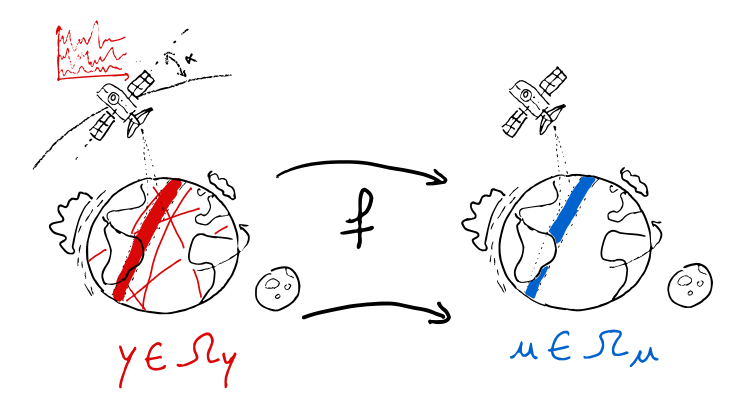
\includegraphics[width=0.8\linewidth]{Chapitre1/Ch1-Figures/Cal_drawing.png} 
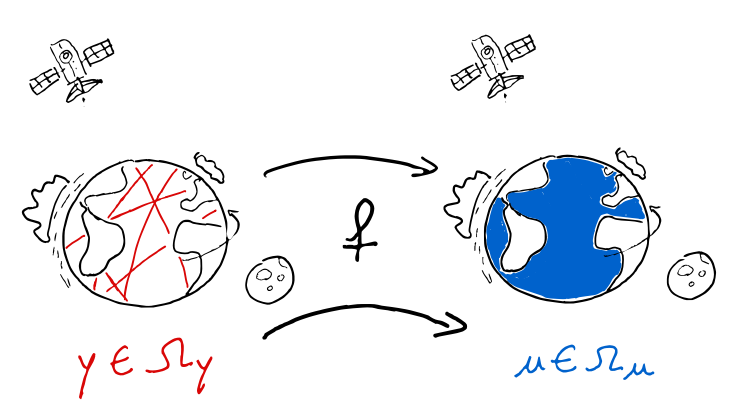
\includegraphics[width=0.8\linewidth]{Chapitre1/Ch1-Figures/Mapping_drawing.png} 
\end{center}
\caption[Swot calibration and altimetry mapping problem illustration]
{\footnotesize The calibration problem (top row) consists in finding the mapping $f$ that estimates the observed SSH $u$ from the SWOT satellite given the actual noisy measurement and ancillary calibrated measures ($y$).
The mapping task (bottom row) consist in finding an operator $f$ that maps partial measurements of the SSH $y$ to a map of SSH $u$}
\label{fig:planet_drawings}
\end{figure}


% \begin{figure}[htbp]
% \begin{center}
% \begin{tabular}[c]
% 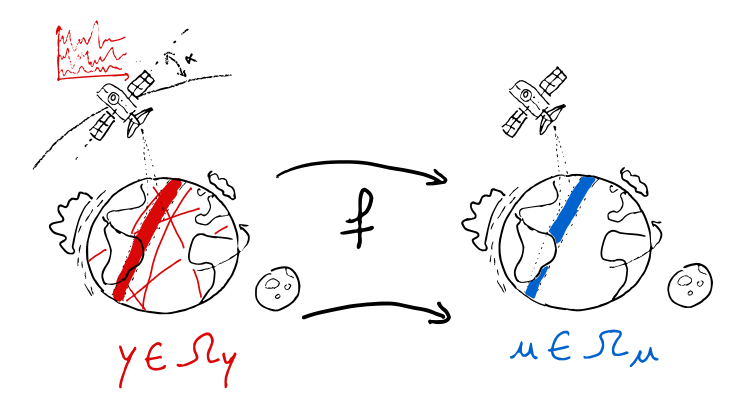
\includegraphics[width=0.8\linewidth]{Chapitre1/Ch1-Figures/Cal_drawing.png} \\
% 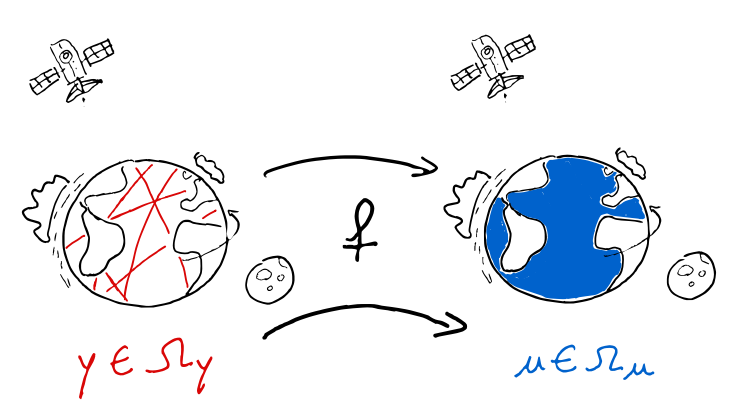
\includegraphics[width=0.8\linewidth]{Chapitre1/Ch1-Figures/Mapping_drawing.png} \\
% \end{tabular}
% \end{center}
% \caption[Swot calibration and altimetry mapping problem illustration]
% {\footnotesize The calibration problem (top row) consists in finding the mapping $f$ that estimates the observed SSH $u$ from the SWOT satellite given the actual noisy measurement and ancillary calibrated measures ($y$).
% The mapping task (bottom row) consist in finding an operator $f$ that maps partial measurements of the SSH $y$ to a map of SSH $u$}
% \label{fig:planet_drawings}
% \end{figure}

\begin{figure}[htbp]
\begin{center}
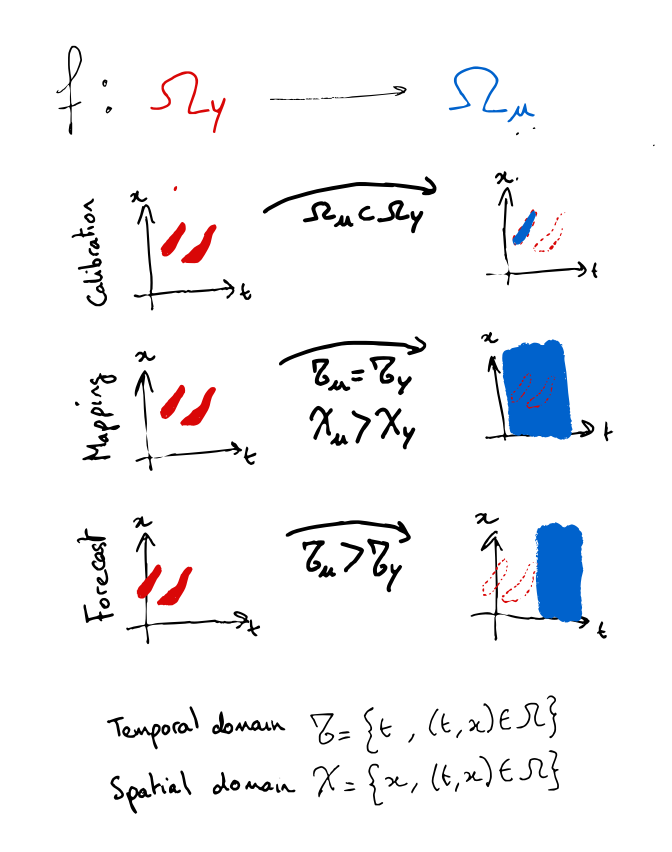
\includegraphics[width=0.8\linewidth]{Chapitre1/Ch1-Figures/Task_ontology.png}
\end{center}
\caption[Task characterization through the domains $\Omega_u$ and $\Omega_y$ of $u$ and $y$]
{\footnotesize Using the perspective provided by the problem definition, we can easily categorize earth observation problems.
The calibration consist of estimating the field $u$ on a subset of the observation domain, the mapping consist in estimating $u$ on the same temporal domain but extending the spatial domain.
And finally forecast can considered as wanting to estimate a quantity on an unobserved future domain.}
\label{fig:task_ontology}
\end{figure}

\section{Method Ontology}
We aim to characterize and organize the various methods used to tackle the class of problem introduced in \ref{sec:chap1_problem_form}. We propose that all methods can be decomposed into the following two steps:
\begin{itemize}
\item Step 1: Define the set $\cal{F}$ of possible $f$ using theoretical knowledge (conceptual models)
\item Step 2: Search $\cal{F}$ for an optimal $f$ using factual knowledge (data)
\end{itemize}

To illustrate our point, consider a simple example of building a thermometer by placing a liquid in a tube and wanting to interpret the level of the liquid as a temperature. According to our previous notations, $y$ is the level of the liquid and $u$ is the temperature of the liquid inside, and we seek to find the mapping $f$ between the two.

Step 1 involves compiling our theoretical knowledge on the problem to define the class of function. Given our understanding of fluid dilation in response to temperature, under the assumption that the diameter of the tube is constant with height, we can state that the level is linearly correlated with the temperature. Therefore, $f$ will be part of $\cal{F} = { y: \alpha y + \beta , (\alpha, \beta) \in |R^2 }$.

In Step 2, to find $\alpha$ and $\beta$, we require two data points to calibrate our model, traditionally obtained by placing the thermometer in icy and boiling water at 1 bar of pressure to get the levels corresponding to 0°C and 100°C. This method relies on strong theoretical foundations and assumptions to reduce the dimensionality of the search space $\cal{F}$, thus facilitating the parameter search with relatively few data points.

However, if we clearly see that the diameter of our thermometer is not constant, the model needs to incorporate that the evolution of the temperature depends on the diameter at each height. This expands the class of functions, necessitating the incorporation of a model of the evolution of the diameter in function of the height, which will introduce new parameters. We could assume that the diameter is linear for every 5mm section, and the corresponding parameters to search would be the value of the diameter every 5mm.

To estimate these new parameters, we need more data which could be direct measures of the diameter or measures of temperature every 5mm. We could directly model $f$ as linear per part, thereby reducing the number of parameters to estimate (no more $\alpha$ and $\beta$). If we have measurements of the temperature, this also alleviates the need to explicitly model the relationship between diameter and temperature.




  
% Tasks
% Simple exemple
% Calibration and mapping example

% Tasks of interests can be summed up as finding f
% Finding f takes two steps: defining the set of possible fs, searching the set for the best f
% Formulating the sets of F requires theoritical knowledge
% Searching the sets of F requires data

% From theory to sets of 
%   inverse problems state x
%   data assimilation: dynamical model
%   spatio temporal correlation: Covariance model
%   deep learning
%   locality: convolution
%   temporal dependence RNN LSTM


Lorem ipsum dolor sit amet, consectetuer adipiscing elit. Maecenas fermentum, elit non lobortis cursus, orci velit suscipit est, id mollis turpis mi eget orci.

\section{Première section du chapitre}

Lorem ipsum dolor sit amet, consectetuer adipiscing elit. Maecenas fermentum, elit non lobortis cursus, orci velit suscipit est, id mollis turpis mi eget orci.

\subsection{Première sous-section}

Lorem ipsum dolor sit amet, consectetuer adipiscing elit. Maecenas fermentum, elit non lobortis cursus, orci velit suscipit est, id mollis turpis mi eget orci.

Voir figure \ref{fig:mafigure2}.


\begin{figure}[htbp]
   \begin{center}
      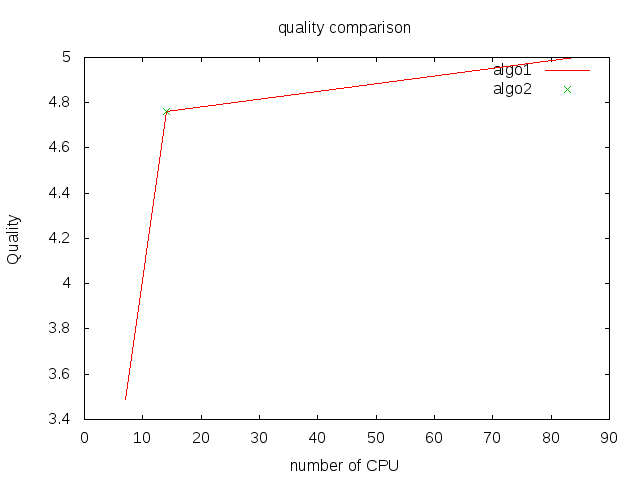
\includegraphics[width=0.8\linewidth]{Chapitre1/Ch1-Figures/comparison.png}
   \end{center}
   \caption[titre court pour la liste des figures]
   {\footnotesize Titre plus long avec des explications.}
   \label{fig:mafigure2}
\end{figure}

\subsection{Deuxième sous-section}

Lorem ipsum dolor sit amet, consectetuer adipiscing elit. Maecenas fermentum, elit non lobortis cursus, orci velit suscipit est, id mollis turpis mi eget orci.

\section{Conclusion du premier chapitre}

Lorem ipsum dolor sit amet, consectetuer adipiscing elit. Maecenas fermentum, elit non lobortis cursus, orci velit suscipit est, id mollis turpis mi eget orci.

In this manuscript I'd like to cite \cite{remo3,remo4}.

\addcontentsline{toc}{section}{Bibliography}
\putbib[./Chapitre1/Ch1-Biblio.bib]
\end{bibunit}


%Input your chapter 2
\clearemptydoublepage
\begin{bibunit}[IEEEtran.bst]

\chapter[SHORT-Nom-du-chapitre-2]{Nom du chapitre 2}
\label{chap:2}

Lorem ipsum dolor sit amet, consectetuer adipiscing elit. Maecenas fermentum, elit non lobortis cursus, orci velit suscipit est, id mollis turpis mi eget orci. 

\section{Première section du chapitre}

\subsection{Première sous-section}

Morbi lorem. Etiam scelerisque rhoncus orci. Nunc elementum ante ac leo. Vestibulum venenatis dictum nunc. Donec turpis est, dictum nec, fringilla nec, cursus id, quam. In nibh orci, porttitor ut, rutrum id, faucibus vitae, leo. Donec ut wisi.

\subsection{Deuxième sous-section}

Lorem ipsum dolor sit amet, consectetuer adipiscing elit. Maecenas fermentum, elit non lobortis cursus, orci velit suscipit est, id mollis turpis mi eget orci. Table \ref{table1}.

\begin{table}[hbt]
\begin{center}
\begin{tabular}{|l|l|l|}
\hline
A & B & C \\ \hline
D & E & F \\ \hline
G & H & I \\ \hline
\end{tabular}
\caption{Test Table}
\label{table1}
\end{center}
\end{table}

\section{Conclusion du second chapitre}

Lorem ipsum dolor sit amet, consectetuer adipiscing elit. Maecenas fermentum, elit non lobortis cursus, orci velit suscipit est, id mollis turpis mi eget orci.

In this manuscript I'd like to cite \cite{remo1,remo5}.

\addcontentsline{toc}{section}{Bibliography}
\putbib[./Chapitre2/Ch2-Biblio.bib]
\end{bibunit}

\clearemptydoublepage
\backmatter
\begin{bibunit}[IEEEtran.bst]

\chapter*{Conclusions and perspectives}
\label{chap:conclusions}
\addcontentsline{toc}{chapter}{Conclusion and perspectives}
\chaptermark{Conclusion}
We review in this chapter the primary contributions outlined in this manuscript and the future avenues of research they open.

\section*{Contributions Summary}
\addcontentsline{toc}{section}{Contributions Summary}
This thesis is part of a broader movement towards developing deep learning methods to address observation challenges in ocean science. It emphasizes altimetry applications, especially in the context of the recent launch of the SWOT mission.

The first contribution highlights the successful application of deep learning for bias correction of simulated SWOT observation data. While standard deep learning architectures struggled to differentiate fine SSH signatures from high amplitude bias, we demonstrated that deep learning methods could be tailored to suit the unique characteristics of altimetry data. We employed SWOT mission's error specifications to craft a custom architecture focused on calibrating SWOT's correlated errors. This study is promising, yet the method developed was calibrated and assessed using simulated data, bringing up questions about its applicability to actual SWOT observations.

The second study delves into how learning-based altimetry methods, once calibrated on simulated data, can be applied to real data. We evaluated the 4dVarNet mapping schemes on real altimetry after calibration on simulated data. The findings indicate strong generalization capabilities even with coarse simulations, while more accurate simulations enhance the mapping performance. The results introduce interesting avenues in exploring the use of numerical simulation for training models for real-world applications.

The initial two studies shed light on the potential of applying learning-based approaches to ocean science's observational challenges. Yet, they also spotlight the complexities in melding expertise in observation, simulation data, deep learning techniques, and domain-specific evaluation methodologies. This spurred the creation of the specialized toolset, Oceanbench, aiming to narrow the gap between deep learning and ocean science experts. Oceanbench enables ocean scientists to flexibly design evaluation setups using data and metrics. These setups come with the essential tools for deep learning practitioners to access and prepare the data in view of training their models. The first iteration presented in this manuscript focuses on sea surface height interpolation but has been thought to be extensible to other ocean observation challenges.

\newpage
\subsection{Current Limitations and perspectives}

Several avenues can be explored to further extend the work presented in this thesis.

\textbf{Small Region \& Period}.
The research presented here pertains to particular region and periods over the Gulfstream which is not representative of the different global regimes. 
This use-case contains a dynamical regime and a well-studied area which has some importance for specific communities and is small enough to mitigate the problems involving scale. 
However confirming the robustness of deep learning schemes on the global ocean is a necessary step to validate their potential.


\textbf{Operational Constraints}.
Real altimetry use-cases involve global and/or high-resolution data. 
This involves dealing with very high-dimensional spatiotemporal global state-space.
In practice, the necessity for the scalability of the method is of paramount importance.
 Transitioning the methods demonstrated in this thesis to functional products would entail considerable scaling challenges. These encompass both scientific aspects, such as dealing with coastlines and varying ocean regimes, and engineering concerns like handling large datasets for the training and assessment of the models.

\textbf{Altimetry as an entrypoint}.
This thesis centers on SSH, a surface field that is relatively well-observed in the realm of ocean quantities. Exploring other quantities, observed through different instrument, with different sampling or even not directly-observed would introduce many more challenges requiring domain-informed problem specifications that deep learning could adress.
Therefore the work presented here is still far away from actual reanalysis and forecasting goals of full state estimation. 
Achieving more ambitious estimation challenge will require a lot of interdisciplinary work across communities and we hope the work done with Oceanbench can help to that regard. 

\textbf{Deep learning interpretability}.
While deep learning methods offer promising results, it's understandable to remain cautious. Concerns regarding the interpretability of deep learning models and their robustness compared to physically descriptive systems are valid points of discussion.
Two potential paths forward can help address these concerns. First, emphasizing the importance of quantifying the uncertainty associated with model estimations. Such uncertainty quantification (UQ) is crucial when addressing ill-posed inverse problems and can play a significant role in bolstering confidence in the results. Second, exploring the realm of physics-informed deep learning and theory-guided datascience, which marries our physical understanding of the ocean with the adaptive nature of deep learning models. Existing studies have dabbled in approaches involving dynamical systems, which, while usually simpler than the ocean, can provide valuable insights for ocean observation applications.

% We review in this chapter the main contributions that have been described in this manuscript as well as the future perspectives introduced through them.

% \section*{Contributions summary}
% \addcontentsline{toc}{section}{Contributions summary}
% Overall this thesis is part of a momentum in developing deep learning methods applied to observation challenges in geosciences.
% More specifically focusing on altimetry applications in the context of the recent lauch of the SWOT mission.

% The first contribution is the successfull of deep learning to bias corrections of simulated SWOT observation data.
% Although off-the-shelf deep learning architectures fail to separate fine SSH signatures from high amplitude bias, we've shown that deep learning methodology can be adapted to the specifities of altimetry data.
% We leveraged SWOT mission's error specifications to design a custom architecture tailored to the calibration of SWOT correlated errrors.
% This study is encouraging but the method developped has been calibrated and evaluated on simulated data, which raises the concerns of applicability to real swot observations.

% The second study shows how learning-based altimetry methods calibrated on simulated data can be applied to real data.
% This is done through the evaluation of 4dVarNet mapping schemes on OSE setups after calibration on simulated data. 
% The results show robust generalization with even coarse simulations while more realistic simulations improve the mapping performances.

% The two first studies opened appealing perspectives for applying learning-based methodology to observation challenges in geosciences.
% However they also highlighted the challenges in combining expertise  observation and simulation data, deep learning methods and domain-informed evaluation procedures.
% This motivated the implementation of an opinionated suite of tools Oceanbench to help bridge the distance between the deep learning and ocean science communities.
% Oceanbench provides a way for ocean scientist to flexibly design evaluation setups with data and metrics. These setups are defined along the necessary tools for deep learning practicioners to train and test their models.


% \section{Perspectives}
% There are a few ways in which the work presented here can extended in interesting ways.

% The element absent from this thesis is the uncertainty quantification which is critical in addressing ill-posed inverse problem. Coming back to the methodological framework introduced in the first chapters, incorporating uncertainty comes down to choosing a probabilistic representation of the estimated SSH.


% This thesis focused on SSH which is a surface field relatively well observed. Other quantities in particular with depth would add significant challenges.

% The evaluations were performed on a specific region, converting the results to operational products would introduce significant scaling challenges, Among which handling coasts and different dynamics.


% Finally, a recurring criticism point to the lack of physical interpretability of deep learning methods. 





% \addcontentsline{toc}{section}{Bibliography}
% \putbib[./Conclusion/End-Biblio.bib]
\end{bibunit}


% \clearemptydoublepage
\addcontentsline{toc}{chapter}{List of publications}

% \chapter*{List of publications}
% \section*{International Journals}
% \section*{International Conferences}

\begin{bibunit}[IEEEtran.bst]
\renewcommand\bibname{List of publications}
\nocite{*}
\putbib[./PublicationList/PubList-Biblio.bib]
\end{bibunit}





\clearemptydoublepage
\begin{bibunit}[IEEEtran.bst]

\chapter*{Appendix}
\addcontentsline{toc}{chapter}{Appendix}

\section*{\textsc{OceanBench}: The Sea Surface Height Edition - Supplementary Material}
% \newpage
% \section{Data Challenges} \label{sec:data_challenges_extended}

In this section, we highlight some details that were omitted in section~\ref{sec:data_challenges}.
This includes details about the simulation type, the data structures, and the training/evaluation periods.

\subsection{OSSE NADIR} \label{sec:osse_nadir}

The reference simulation is the \textit{NATL60} simulation based on the NEMO model~\cite{NEMOAJAYI2020}. 
This particular simulation was run over an entire year without any tidal forcing.
The simulation provides the outputs of SSH, SST, sea surface salinity (SSS) and the u,v velocities every 1 hour.
For the purposes of this data challenge, the spatial domain is over the Gulfstream with a spatial domain of $[-65^\circ, -55^\circ]$ longitude and $[33^\circ, 43^\circ]$ latitude.
The resolution of the original simulation is 1/60$^\circ$ resolution with hourly snapshots, and we consider a daily downsampled trajectory at 1/20$^\circ$ for the data challenge which results in a 365x200x200 spatio-temporal grid.
This simulation resolves finescale dynamical processes ($\sim$15km) which makes it a good test bed for creating an OSSE environment for mapping.
The SSH observations include simulations of ocean satellite NADIR tracks.
In particular, they are simulations of Topex-Poseidon, Jason 1, Geosat Follow-On, and Envisat.
There is no observation error considered within the challenge.
We use a the entire period from 2012-10-10 until 2013-09-30.
A training period is only from 2013-01-02 to 2013-09-30 where the users can use the reference simulation as well as all available simulated observations.
The evaluation period is from 2012-10-22 to 2012-12-02 (i.e. 41 days) which is considered decorrelated from the training period. 
During the evaluation period, the user cannot use the reference NATL60 simulation but they can use all available simulated observations. There is also a spin-up period allowance from 2012-10-01 where the user can also use all available simulated observations.

\subsection{OSSE SWOT \& OSSE SST} \label{sec:osse_swot_sst}

For the OSSE SWOT and OSSE SST experiments, the reference simulation, domain, and evaluation period is the same as the OSSE NADIR experiment.
However, the OSSE SWOT includes simulated observations of the novel KaRIN sensor recently deployed during the SWOT mission, the pseudo-observations were generated using the SWOT simulator~\cite{SWOT}. 
This OSSE SST experiment allows the users to utilize the full fields of SST as inputs to help reconstruct the SSH field in conjunction with the NADIR and SWOT SSH observation.
Because the SST comes from the same NATL60 simulation, the geometry characteristics SST and SSH are exactly the same.

\subsection{OSE NADIR} \label{sec:ose_nadir}

The OSE NADIR experiment only uses real observations aggregated from different altimeters. These SSH observations include observations from the SARAL/Altika, Jason 2, Jason 3, Sentinel 3A, Haiyang-2A and Cryosat-2 altimeters. The Cryosat-2 altimeter is used as the independent evaluation track used to assess the performance of the reconstructed SSH field.

\subsection{Results}

We use \texttt{OceanBench} to generate maps of relevant quantities from the 4DVarNet method~\cite{4DVARNETSWOT,4DVARNETSST}.
Figure~\ref{fig:oceanbench_maps_4dvarnet} showcases some demo maps for some key physical variables outlined in section~\ref{sec:physical_variables}.
We showcase the 4DVarNet method because it is the SOTA method that was applied to each of the data challenges.
We can see that the addition of more information, i.e. NADIR -> SWOT -> SST, results in maps look more similar to the NEMO simulation in the OSSE challenges.
It also produces sensible maps for the OSE challenge as well.

\texttt{OceanBench} also generated figure~\ref{fig:oceanbench_psd_4dvarnet} which shows plots of the PSD and PSD scores of SSH for the different challenges.
Again, as we increase the efficacy of the observations via SWOT and allow for more external factors like the SST, we get an improvement in the isotropic and spacetime PSD scores.
In addition, we see that the PSD plots for the OSE task look very similar to the OSE challenges. 

Lastly, we used \texttt{OceanBench} to generate a leaderboard of metrics for a diverse set of algorithms where the maps were available online.
Table~\ref{tb:exp-results-mega} displays all of the key metrics outlined in section~\ref{sec:metrics} including the normalized RMSE and various spectral scores which are appropriate for the challenge.
We see that as the complexity of the method increases, the metrics improve. 
In addition, the methods that involve end-to-end learning perform the best overall, i.e. 4DVarNet.

\begin{figure}[ht!]
\small
\begin{center}
\setlength{\tabcolsep}{1pt}
\begin{tabular}{cccc}
\hspace{3mm} Task OSSE & 
\hspace{3mm} Task OSSE & 
\hspace{2mm} Task OSSE & 
Task OSE \\
\hspace{3mm}  Nadir & 
\hspace{3mm} Nadir + SWOT & 
\hspace{2mm} Nadir + SST & 
Nadir \\
%\vspace{-2mm}
%%%%% SSH %%%%%%%%
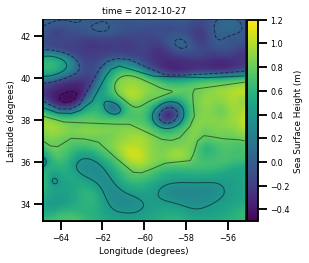
\includegraphics[trim={0 13mm 22mm 0},clip, width=3.60cm,height=3.2cm]{content/figures/fourdvarnet_figs/osse_gf_nadir_ssh.png} &
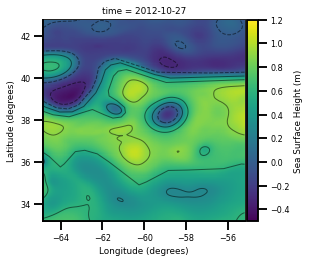
\includegraphics[trim={13mm 13mm 22mm 0},clip, width=3.2cm,height=3.2cm]{content/figures/fourdvarnet_figs/osse_gf_nadirswot_ssh.png} &
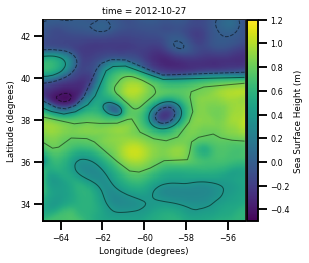
\includegraphics[trim={13mm 13mm 22mm 0},clip, width=3.2cm,height=3.2cm]{content/figures/fourdvarnet_figs/osse_gf_nadir_sst_ssh.png} &
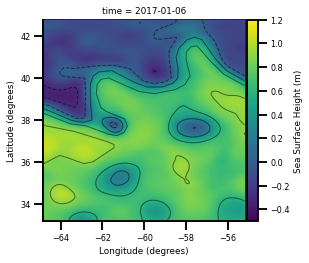
\includegraphics[trim={13mm 13mm 0 0},clip,width=4.0cm,height=3.2cm]{content/figures/fourdvarnet_figs/ose_gf_ssh.png} \\
%\vspace{3mm}
%%%%% KINETIC ENERGY %%%%%%%%
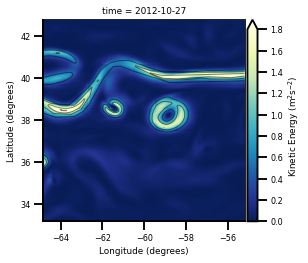
\includegraphics[trim={0 13mm 22mm 5mm}, clip, width=3.60cm,height=3cm]{content/figures/fourdvarnet_figs/osse_gf_nadir_ke.png} &
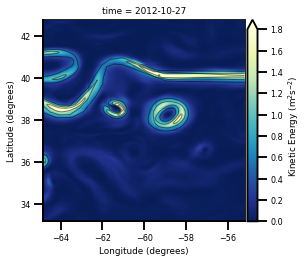
\includegraphics[trim={13mm 13mm 22mm 5mm},clip, width=3.2cm,height=3cm]{content/figures/fourdvarnet_figs/osse_gf_nadirswot_ke.png} &
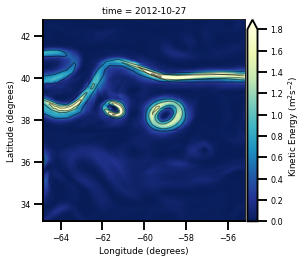
\includegraphics[trim={13mm 13mm 22mm 5mm},clip, width=3.2cm,height=3cm]{content/figures/fourdvarnet_figs/osse_gf_nadir_sst_ke.png} &
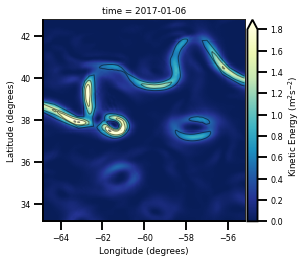
\includegraphics[trim={13mm 13mm 0 5mm},clip,width=4cm,height=3cm]{content/figures/fourdvarnet_figs/ose_gf_ke.png} \\
%%%%% RELATIVE VORTICITY %%%%%%%%
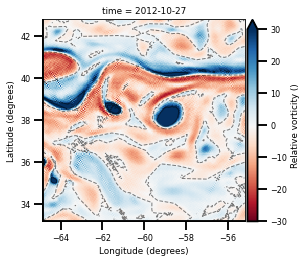
\includegraphics[trim={0 13mm 21.2mm 5mm},clip, width=3.60cm,height=3cm]{content/figures/fourdvarnet_figs/osse_gf_nadir_vort_r.png} &
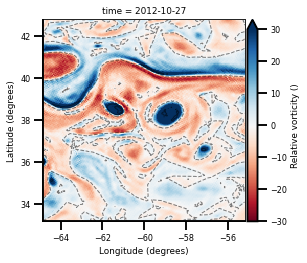
\includegraphics[trim={13mm 13mm 21.2mm 5mm},clip, width=3.2cm,height=3cm]{content/figures/fourdvarnet_figs/osse_gf_nadirswot_vort_r.png} &
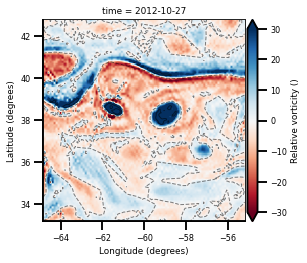
\includegraphics[trim={13mm 13mm 21.2mm 5mm},clip, width=3.2cm,height=3cm]{content/figures/fourdvarnet_figs/osse_gf_nadir_sst_vort_r.png} &
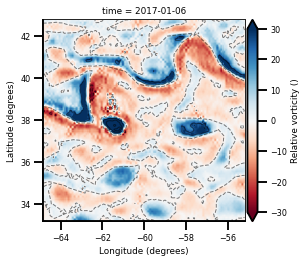
\includegraphics[trim={13mm 13mm 0 5mm},clip,width=4.0cm,height=3cm]{content/figures/fourdvarnet_figs/ose_gf_vort_r.png} \\
%%%%% STRAIN %%%%%%%%
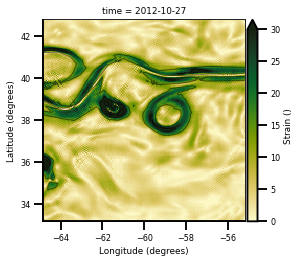
\includegraphics[trim={0 0 19mm 5mm},clip, width=3.60cm,height=3.4cm]{content/figures/fourdvarnet_figs/osse_gf_nadir_strain.png} &
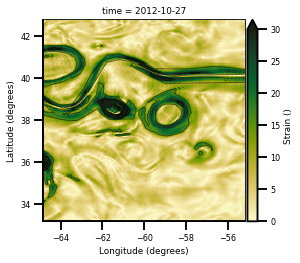
\includegraphics[trim={13mm 0 19mm 5mm},clip, width=3.2cm,height=3.4cm]{content/figures/fourdvarnet_figs/osse_gf_nadirswot_strain.png} &
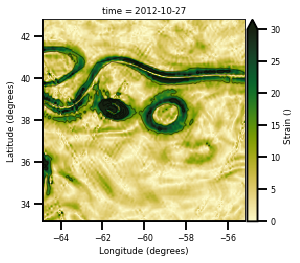
\includegraphics[trim={13mm 0 19mm 5mm},clip, width=3.2cm,height=3.4cm]{content/figures/fourdvarnet_figs/osse_gf_nadir_sst_strain.png} &
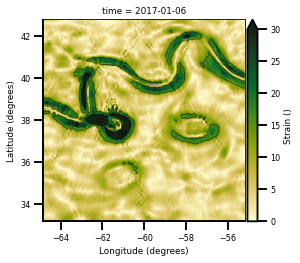
\includegraphics[trim={13mm 0 0 5mm},clip,width=4.0cm,height=3.4cm]{content/figures/fourdvarnet_figs/ose_gf_strain.png} \\
% \vspace{-2mm}
(a) & (b) & (c) & (d)
\end{tabular}
\vspace{-3mm}
% \caption{Row I - Isotrophic PSD. Row 2 - Isotrophic PSD Score}
\caption{
Reconstructed quantities by the 4dVarNet method for each of the four tasks.
Each row showcases the following physical variables found in appendix~\ref{sec:physical_variables}: (a) Sea Surface Height, (b) Kinetic Energy, (c) Relative Vorticity, and (d) Strain. 
Each column showcase the reconstructed from the tasks (a) OSSE using only Nadir tracks: (b) OSSE using Nadir tracks and SWOT swath, (c) Multimodal using Nadir tracks and sea surface temperature, and (d) Reconstruction using real nadir altimetry tracks.}
\vspace{-5mm}
\label{fig:oceanbench_maps_4dvarnet}
\end{center}
\end{figure}





% \begin{figure}[ht!]
\small
\begin{center}
\setlength{\tabcolsep}{1pt}
\begin{tabular}{cccc}
\hspace{3mm} Task OSSE & 
\hspace{3mm} Task OSSE & 
\hspace{2mm} Task OSSE & 
Task OSE \\
\hspace{3mm}  Nadir & 
\hspace{3mm} Nadir + SWOT & 
\hspace{2mm} Nadir + SST & 
Nadir \\
%\vspace{-2mm}
%%%%% SSH %%%%%%%%
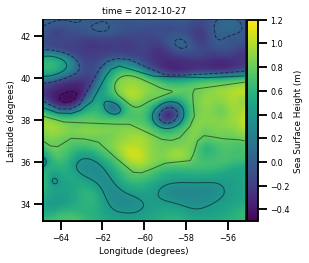
\includegraphics[trim={0 13mm 22mm 0},clip, width=3.60cm,height=3.2cm]{content/figures/fourdvarnet_figs/osse_gf_nadir_ssh.png} &
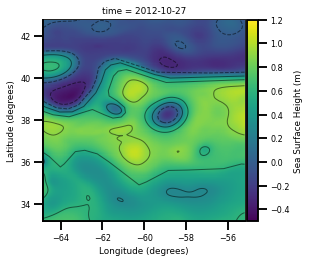
\includegraphics[trim={13mm 13mm 22mm 0},clip, width=3.2cm,height=3.2cm]{content/figures/fourdvarnet_figs/osse_gf_nadirswot_ssh.png} &
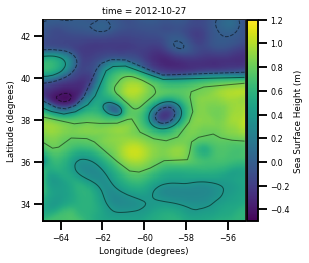
\includegraphics[trim={13mm 13mm 22mm 0},clip, width=3.2cm,height=3.2cm]{content/figures/fourdvarnet_figs/osse_gf_nadir_sst_ssh.png} &
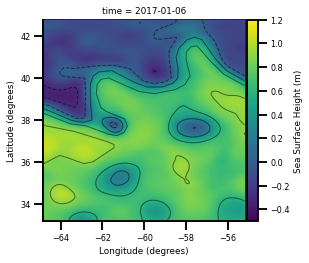
\includegraphics[trim={13mm 13mm 0 0},clip,width=4.0cm,height=3.2cm]{content/figures/fourdvarnet_figs/ose_gf_ssh.png} \\
%\vspace{3mm}
%%%%% KINETIC ENERGY %%%%%%%%
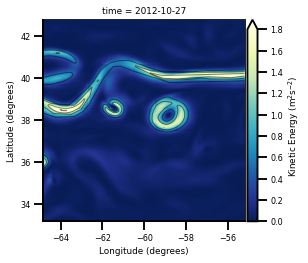
\includegraphics[trim={0 13mm 22mm 5mm}, clip, width=3.60cm,height=3cm]{content/figures/fourdvarnet_figs/osse_gf_nadir_ke.png} &
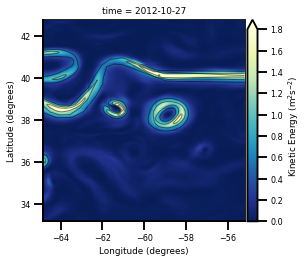
\includegraphics[trim={13mm 13mm 22mm 5mm},clip, width=3.2cm,height=3cm]{content/figures/fourdvarnet_figs/osse_gf_nadirswot_ke.png} &
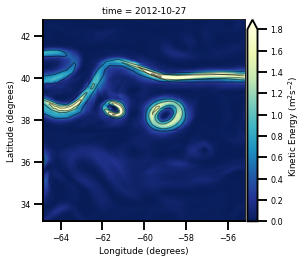
\includegraphics[trim={13mm 13mm 22mm 5mm},clip, width=3.2cm,height=3cm]{content/figures/fourdvarnet_figs/osse_gf_nadir_sst_ke.png} &
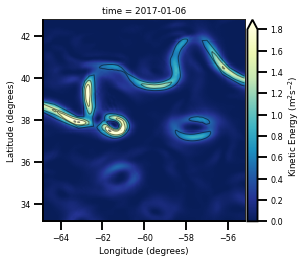
\includegraphics[trim={13mm 13mm 0 5mm},clip,width=4cm,height=3cm]{content/figures/fourdvarnet_figs/ose_gf_ke.png} \\
%%%%% RELATIVE VORTICITY %%%%%%%%
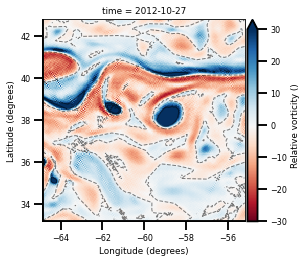
\includegraphics[trim={0 13mm 21.2mm 5mm},clip, width=3.60cm,height=3cm]{content/figures/fourdvarnet_figs/osse_gf_nadir_vort_r.png} &
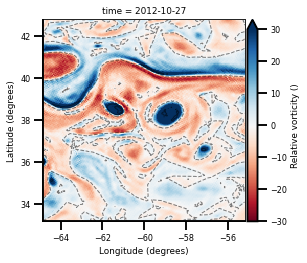
\includegraphics[trim={13mm 13mm 21.2mm 5mm},clip, width=3.2cm,height=3cm]{content/figures/fourdvarnet_figs/osse_gf_nadirswot_vort_r.png} &
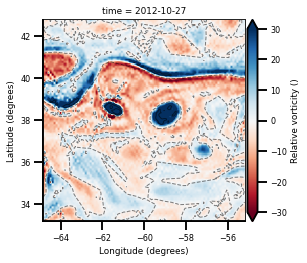
\includegraphics[trim={13mm 13mm 21.2mm 5mm},clip, width=3.2cm,height=3cm]{content/figures/fourdvarnet_figs/osse_gf_nadir_sst_vort_r.png} &
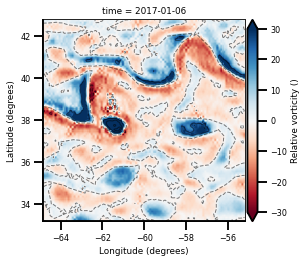
\includegraphics[trim={13mm 13mm 0 5mm},clip,width=4.0cm,height=3cm]{content/figures/fourdvarnet_figs/ose_gf_vort_r.png} \\
%%%%% STRAIN %%%%%%%%
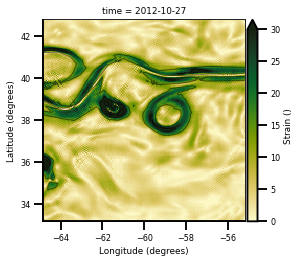
\includegraphics[trim={0 0 19mm 5mm},clip, width=3.60cm,height=3.4cm]{content/figures/fourdvarnet_figs/osse_gf_nadir_strain.png} &
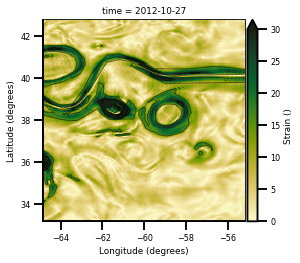
\includegraphics[trim={13mm 0 19mm 5mm},clip, width=3.2cm,height=3.4cm]{content/figures/fourdvarnet_figs/osse_gf_nadirswot_strain.png} &
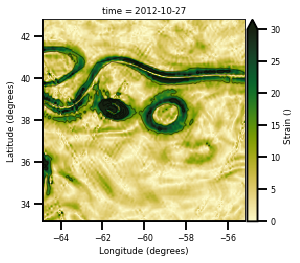
\includegraphics[trim={13mm 0 19mm 5mm},clip, width=3.2cm,height=3.4cm]{content/figures/fourdvarnet_figs/osse_gf_nadir_sst_strain.png} &
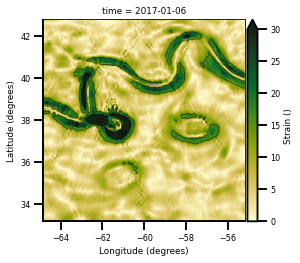
\includegraphics[trim={13mm 0 0 5mm},clip,width=4.0cm,height=3.4cm]{content/figures/fourdvarnet_figs/ose_gf_strain.png} \\
% \vspace{-2mm}
(a) & (b) & (c) & (d)
\end{tabular}
\vspace{-3mm}
% \caption{Row I - Isotrophic PSD. Row 2 - Isotrophic PSD Score}
\caption{
Reconstructed quantities by the 4dVarNet method for each of the four tasks.
Each row showcases the following physical variables found in appendix~\ref{sec:physical_variables}: (a) Sea Surface Height, (b) Kinetic Energy, (c) Relative Vorticity, and (d) Strain. 
Each column showcase the reconstructed from the tasks (a) OSSE using only Nadir tracks: (b) OSSE using Nadir tracks and SWOT swath, (c) Multimodal using Nadir tracks and sea surface temperature, and (d) Reconstruction using real nadir altimetry tracks.}
\vspace{-5mm}
\label{fig:oceanbench_maps_4dvarnet}
\end{center}
\end{figure}


\begin{table}[ht]
\caption{This table showcases all of the summary statistics for some methods for each of the data challenges listed in section~\ref{sec:data_challenges} and~\ref{sec:data_challenges_extended}. The summary statistics shown are the normalized RMSE and the effective resolution in the spectral domain. The spectral metrics for the effective resolution that were outlined in section~\ref{sec:metrics} are: i) $\lambda_a$ is the spatial score for the alongtrack PSD score, ii) $\lambda_r$ is the spatial score for the isotropic PSD, iii) $\lambda_x$ is the spatial score for space-time PSD score, and iv) $\lambda_t$ is the temporal score for the space-time PSD score.}
% \caption{This table highlights some of the results for the OSSE experiments outlined in section~\ref{sec:osse} and~\ref{sec:other_tasks}.

% This table highlights the performance statistically in the real and spectral space; the normalized RMSE for the real space and the minimum spatial and temporal scales resolved in the spectral domain. 
% For more information about the class of models displayed and class of metrics, see section~\ref{sec:ml_ontology} and section~\ref{sec:metrics} respectively.}
\label{tb:exp-results-mega}
\centering
\begin{tabular}{llcccccc}
 \toprule
% Experiment & Configuration & Method & nRMSE & Resolved Scale [km]    \\ \midrule
% \multirow{2}{*}{Experiment} & \multirow{2}{*}{Algorithm} & \multirow{2}{*}{Algorithm Class} & \multirow{2}{*}{nRMSE} & \multicolumn{2}{c}{Effective Resolution} \\ 
% &  &   &  & Wavelength [km]  & Period [days]      \\ \midrule
% \multirow{2}{*}{Experiment} & \multirow{2}{*}{Algorithm} & \multirow{2}{*}{Algorithm Class} & \multirow{2}{*}{nRMSE} & \multicolumn{2}{c}{Effective Resolution} \\ 
\multirow{2}{*}{Experiment} &  \multirow{2}{*}{Algorithm} &   \multirow{2}{*}{nRMSE Score} &
\multicolumn{4}{c}{Effective Resolution} \\
& & & $\lambda_{a}$ [km] & $\lambda_{r}$ [km]   &  $\lambda_{\mathbf{x}}$ [km]  &   $\lambda_{t}$ [days]      \\ \midrule
OSSE NADIR     &  OI & 0.92 & - & 123 & 174 & 10.8 \\
OSSE NADIR     &  MIOST &  0.93 & - & 100 & 157 & 10.1 \\
OSSE NADIR     &  BFNQG & 0.93 & - & 88 & 139 & 10.4 \\
OSSE NADIR &  4DVarNet &  \textbf{0.94} & - & \textbf{65} & \textbf{117} & \textbf{7.7} \\
\midrule
OSSE SWOT     &  OI & 0.92 & - & 106 & 139 & 11.7 \\
OSSE SWOT     &  MIOST &  0.94 & - & 88 & 131 & 10.1 \\
OSSE SWOT     &  BFNQG & 0.94 & - & 64 & 118 & 36.5 \\
OSSE SWOT &  4DVarNet &  \textbf{0.96} & - & \textbf{47} & \textbf{77} & \textbf{5.6} \\
\midrule
OSSE SST     &  Musti & 0.95 & - & 46 & 138 & 4.1 \\
OSSE SST &  4DVarNet &  \textbf{0.96} & - & \textbf{46} & \textbf{87} & \textbf{3.7} \\
\midrule
OSE NADIR     &  OI & 0.88 & 151 & - &  - &  -\\
OSE NADIR     &  MIOST &  0.90 & 135 & - &  - &  -\\
OSE NADIR     &  BFNQG & 0.88 & 122 & - & - &  -\\
OSE NADIR &  ConvLSTM &  0.89 & 113 &- &  - &  -\\
OSE NADIR &  4DVarNet & \textbf{0.91} & \textbf{98} & - &  -  &  -\\
\bottomrule
\end{tabular}
\end{table}

% \subsection{Simulated Altimetry Tracks} \label{sec:dc_osse_nadir}

% \textcolor{red}{
% The most commonly used SSH maps, the Developing Use of Altimetry for Climate Studies (DUACS) products, are derived from a statistical space–time interpolation of nadir altimeter observations. This intrinsically limits the effective resolution [as defined in Skamarock (2004), i.e., the fully resolved scales] of DUACS SSH maps to 150–200 km at middle latitudes (Ballarotta et al. 2019). The SSH mapping algorithm was developed by CNES and CLS in 1997, as part of the DUACS project, and has been continuously improved since then (Taburet et al. 2019). The DUACS products are now distributed by the Copernicus Marine Environment Monitoring Service (CMEMS). DUACS algorithm implements a statistical interpolation of SSH satellite data in space and time to produce global daily maps (Le Traon et al. 1998). The data are collected by a constellation of 2 to 4 nadir-looking altimeters (sometimes referred to as conventional altimeters), and characterized by large data gaps reaching 200 km in the zonal direction at the equator.
% }

% \subsection{Simulated SWOT Tracks} \label{sec:dc_osse_swot}


% \textcolor{red}{
% The Surface Water and Ocean Topography (SWOT; Fu et al. 2012; Morrow et al. 2019) altimetry mission, to be launched in early 2022, will open the way to SSH maps with resolution significantly higher than 150 km at midlatitudes, but this perspective entails a thorough revisit of the mapping algorithm. SWOT will considerably increase the measurement density at the surface of the oceans thanks to SSH measurements at a kilometric pixel resolution over a swath 120 km wide. On the swath, SWOT is expected to resolve scales down to 15 km at low latitude and 30–45 km at mid- and high latitudes (Wang et al. 2019). In its science phase, SWOT will have a 21 days repeat orbit, allowing an average revisit time of 11 days in most of the globe. Some of the dynamical processes observable by SWOT evolve over time scales on the order of 1 day, much shorter than the satellite revisit time. Consequently, the mapping method implemented in the current DUACS system will certainly not be sufficient to draw the maximum benefit from SWOT. A linear interpolation will filter most of the observed small-scale signals between two passes of the satellite, as anticipated by Gaultier et al. (2016).These authors advocate for using more advanced methods to build SSH maps.
% }

% \subsection{Multimodal with Sea Surface Temperature}  \label{sec:dc_osse_sst}


% \subsection{Real Altimetry Tracks}  \label{sec:dc_ose_nadir}

\subsection{Datasets} \label{sec:datasets}

In Table~\ref{tb:datasets-mega}, we showcase all of the available datasets in our\footnote{Available at: \href{https://github.com/quentinf00/oceanbench-data-registry}{OceanBench Data Registry}} for the challenges listed in the above section. The license for the datasets listed in the registry are under the CCA 4.0 International License.

\begin{landscape}
\begin{table}[ht]
\caption{This table gives an extended overview of the datasets provided to complete the data challenges listed in~\ref{sec:data_challenges} and~\ref{sec:data_challenges_extended}. The OSSE SST and SSH are outputs from come from the free run NEMO model~\citep{NEMOAJAYI2020}. The OSSE NADIR and SWOT are pseudo-observations generated from the NEMO simulation. We provide the original simulated satellite tracks as well as a gridded version at the same resolution as the simulation. 
}
\label{tb:datasets-mega}
\centering
\begin{tabular}{lcclclcc}
 \toprule
     & OSSE SSH      & \multicolumn{2}{c}{OSSE SSH NADIR}                     & \multicolumn{2}{c}{OSSE SSH SWOT}                      & OSSE SST             & OSE SSH NADIR            \\ \midrule\midrule
Data Structure & Gridded              & AlongTrack           & \multicolumn{1}{c}{Gridded} & AlongTrack           & \multicolumn{1}{c}{Gridded} & Gridded              & AlongTrack           \\
     & \multicolumn{1}{l}{} & \multicolumn{1}{l}{} &                             & \multicolumn{1}{l}{} &  \\ \midrule
Source     & 
NEMO~\citep{NEMOAJAYI2020} &
NEMO~\citep{NEMOAJAYI2020} &
NEMO~\citep{NEMOAJAYI2020} &
NEMO~\citep{NEMOAJAYI2020} & 
NEMO~\citep{NEMOAJAYI2020} &
NEMO~\citep{NEMOAJAYI2020}
% \multicolumn{3}{c}{NEMO GCM\citep{NEMOAJAYI2020}}  
& Altimetry~\citep{MDSALONGTRACK} \\
Region & 
GulfStream & GulfStream & GulfStream & GulfStream &
GulfStream & GulfStream & GulfStream
\\
Domain Size [degrees] &
% ($L_x\times L_y$) 
$10\times 10^\circ$ &
$10\times 10^\circ$ &
$10\times 10^\circ$ &
$10\times 10^\circ$ &
$10\times 10^\circ$ &
$10\times 10^\circ$ &
$10\times 10^\circ$ \\
Domain Size [km] &
% ($L_x\times L_y$) 
$1,100\times 1,100$ &
$1,100\times 1,100$ &
$1,100\times 1,100$ &
$1,100\times 1,100$ &
$1,100\times 1,100$ &
$1,100\times 1,100$ &
$1,100\times 1,100$ \\
Longitude Extent &
$[-65^\circ, -55^\circ]$ & 
$[-65^\circ, -55^\circ]$ & 
$[-65^\circ, -55^\circ]$ & 
$[-65^\circ, -55^\circ]$ & 
$[-65^\circ, -55^\circ]$ &
$[-65^\circ, -55^\circ]$ &
$[-65^\circ, -55^\circ]$ \\
Latitude Extent &
$[33^\circ, 43^\circ]$ &
$[33^\circ, 43^\circ]$ &
$[33^\circ, 43^\circ]$ &
$[33^\circ, 43^\circ]$ &
$[33^\circ, 43^\circ]$ &
$[33^\circ, 43^\circ]$ &
$[33^\circ, 43^\circ]$ \\
Resolution [degrees] &
% ($\Delta_x\times \Delta_y$) 
$0.05^\circ\times 0.05^\circ$ &
N/A &
$0.05^\circ\times 0.05^\circ$ &
N/A &
$0.05^\circ\times 0.05^\circ$ &
$0.05^\circ\times 0.05^\circ$ &
N/A \\
Resolution [km] &
% ($\Delta_x\times \Delta_y$) 
$5.5\times 5.5$ &
$6$ &
$5.5\times 5.5$ &
$6$ &
$5.5\times 5.5$ &
$5.5\times 5.5$ &
$7$ \\
Grid Size &
$200\times 200$ & 
N/A &
$200\times 200$ & 
N/A &
$200\times 200$ & 
$200\times 200$ & 
N/A \\
Num. Datapoints &
$\sim$14.6M & 
$\sim$205K & 
$\sim$14.6M & 
$\sim$955K & 
$\sim$14.6M & 
$\sim$14.6M & 
$\sim$1.79M \\ \midrule
Period Start & 
2012-10-01 & 2012-10-01 & 2012-10-01 & 2012-10-01 & 
2012-10-01 & 2012-10-01 & 2016-12-01 \\
Period End & 
2013-09-30 & 2013-09-30 & 2013-09-30 & 2013-09-30 & 
2013-09-30 & 2013-09-30 & 2018-01-31 \\
Frequency  & 
Daily & 1 Hz  & Daily & 1 Hz  & Daily & Daily & 1 Hz \\ 
Period Length & 365 Days & 365 Days & 365 Days &
365 Days & 365 Days & 365 Days & 427 Days \\
\midrule
Evaluation Start & 
2012-10-22 & 2012-10-22 & 2012-10-22 & 2012-10-22 & 
2012-10-22 & 2012-10-22 & 2017-01-01 \\
Evaluation End & 
2012-12-02 & 2012-12-02 & 2012-12-02 & 2012-12-02 & 
2012-12-02 & 2012-12-02 & 2017-12-31 \\ 
Evaluation Length & 45 Days & 45 Days & 45 Days &
45 Days & 45 Days & 45 Days & 365 Days \\
\bottomrule
\end{tabular}
\end{table}
\end{landscape}
% \newpage
\section{Physical Variables} \label{sec:physical_variables}

As alluded to in the main body of the paper, we have access to many physical quantities which can be derived from  sea surface height. 
This gives us a way to analyze how effective and trustworthy are our reconstructions. 
Many machine learning methods are unconstrained so they may provide solutions that are physically inconsistent and visualizing the field is a very easy eye test to assess the validity. 
In addition to post analysis, one could include some of these derived quantities maybe useful as additional inputs to the system and/or constraints to the loss function. 




% \begin{table}[h!]
%   \caption{Table of nomanclature}
%   \label{sample-table}
%   \centering
%   \begin{tabular}{ccl}
%     \toprule
%     Symbol & Size & Description  \\
%     \midrule
%     $\mathbf{x}_s$ & $\mathbb{R}^{D_s}$ & Spatial Coordinates  \\
%     $t$ & $\mathbb{R}^{D_t}$ & Temporal Coordinates  \\
%    $\boldsymbol{f}(\mathbf{x}_s, t)$ & $\mathbb{R}^{D}$ & Spatiotemporal Field  \\
%    $\boldsymbol{y}_{obs}(\mathbf{x}_s, t)$ & $\mathbb{R}^{D_{obs}}$ & Spatiotemporal Observations  \\
%    $\eta$ & $\mathbb{R}$ & Sea Surface Height $[m]$ \\
%    $\bar{\eta}$ & $\mathbb{R}$ & Sea Surface Anomaly $[m]$ \\
%    $u$ & $\mathbb{R}$ & Zonal Velocity $[ms^{-2}]$ \\
%    $v$ & $\mathbb{R}$ & Meridional Velocity $[ms^{-2}]$ \\
%     \bottomrule
%   \end{tabular}
%   \label{tb:notation}
%  \end{table}


% \subsection{Coordinates}
% \textbf{SpatioTemporal Coordiantes}. We define some generic spatiotemporal coordinates.
% 
% We are dealing with satellite observations, so we are interested in the domain across the Earth's surface. 
% Let us define the Earth's domain by some spatial coordinates, $\mathbf{x} = [\text{Longitude},\text{Latitude}]^\top \in\mathbb{R}^{D_s}$, and temporal coordinates, $t=[\text{Time}]\in\mathbb{R}^+$, where $D_s$ is the dimensionality of the coordinate vector.  
% We can define some spatial (sub-)domain, $\Omega\subseteq\mathbb{R}^{D_s}$, and a temporal (sub-)domain, $\mathcal{T}\subseteq\mathbb{R}^+$. 
% This domain could be the entire globe for 10 years or a small region within the North Atlantic for 1 year.
%
%
% \begin{align} \label{eq:spatiotemporal_coords}
%     \text{Spatial Coordinates}: && \mathbf{x} &\in \Omega \subseteq \mathbb{R}^{D_s}\\ 
%     \text{Temporal Coordinates}: && t &\in \mathcal{T} \subseteq \mathbb{R}^{D_t}.
% \end{align}
% %
%
% In this case $D_s=2$ because we only have a two coordinates, however we can do some coordinate transformations like spherical to Cartesian. Likewise, we can do some coordinate transformation for the temporal coordinates like cyclic transformations or sinusoidal embeddings~\cite{ATTENTION}. We have two fields of interest from these spatiotemporal coordinates: the state and the observations.
% %
% %
% \begin{align} \label{eq:state_obs}
%     \text{State}: && \boldsymbol{u}(\mathbf{x},t) &: \Omega\times\mathcal{T}\rightarrow\mathbb{R}^{D_u} \\
%     \text{Observations}: && \boldsymbol{y}_{obs}(\mathbf{x},t) &: \Omega\times\mathcal{T}\rightarrow\mathbb{R}^{D_{obs}}
% \end{align}
% %
% %
% The state domain, $u\in\mathcal{U}$, is a scalar or vector-valued field of size $D_u$ which is typically the quantity of interest and the observation domain, $y_{obs}\in\mathcal{Y}_{obs}$, is the observable quantity which is also a scalar or vector-valued field of size $D_{obs}$. Now, we make the assumption that we have an operator $\mathcal{H}$ that transforms the field from the state space, $\boldsymbol{u}$, to the observation space, $\boldsymbol{y}_{obs}$.
% %
% %
% \begin{align} \label{eq:prob_definition}
%     \boldsymbol{y}_{obs}(\mathbf{x},t) = \mathcal{H}\left(\boldsymbol{u}(\mathbf{x},t), t, \boldsymbol{\varepsilon}, \boldsymbol{\mu}\right) 
% \end{align}
% %
% %


% % \subsection{Field}

% \textbf{Field}. We have the generic definition of a scalar or vector-valued field.

% \begin{align} \label{eq:field}
% \text{Field}:&& f&=\boldsymbol{f}(\mathbf{x},t), && \quad \Omega\times \mathcal{T}\rightarrow\mathbb{R}^{D}
% \end{align}



Recall the spatiotemporal coordinates from equation~\ref{eq:spatiotemporal_coords}, 
we use the same coordinates for the subsequent physical quantities. \textbf{Sea Surface Height} is the deviation of the height of the ocean surface from the geoid of the Earth. We can define it as:
%
\begin{align}
	\text{Sea Surface Height }[m]:&& \quad
 \eta &= \boldsymbol{\eta}(\mathbf{x},t)&& \quad \Omega\times \mathcal{T}\rightarrow\mathbb{R} \label{eq:ssh}
\end{align}
%
This quantity is the actual value that is given from the satellite altimeters and is presented in the products for SSH maps~\cite{DUACS}. An example can be seen in the first row of figure~\ref{fig:oceanbench_maps_4dvarnet}.
%
\textbf{Sea Surface Anomaly} is the anomaly wrt to the spatial mean which is defined by
%
\begin{align}
	\text{Sea Level Anomaly }[m]:&& \quad
 \bar{\eta} &= \boldsymbol{\eta}(\mathbf{x},t) - \bar{\eta}(t) &&
 \quad \Omega\times \mathcal{T}\rightarrow\mathbb{R} \label{eq:sla}
\end{align}
%
where $\bar{\eta}(t)$ is the spatial average of the field at each time step.  
An example can be seen in the first row of figure~\ref{fig:oceanbench_maps}.
%
Another important quantity is the \textbf{geostrophic velocities} in the zonal and meridional directions. This is given by
%
\begin{align}
	\text{Zonal Velocity}[ms^{-2}]:&& \quad
 u &= -\frac{g}{f_0}\frac{\partial \eta}{\partial y} &&
 \quad \Omega\times \mathcal{T}\rightarrow\mathbb{R} \label{eq:u_vel} \\
	\text{Meridional Velocity}[ms^{-2}]:&& \quad
 v &= \frac{g}{f_0}\frac{\partial \eta}{\partial x} &&
 \quad \Omega\times \mathcal{T}\rightarrow\mathbb{R} \label{eq:v_vel}
\end{align}
% 
where $g$ is the gravitational constant and $f_0$ is the mean Coriolis parameter. These quantities are important as they can be an related to the sea surface current. The geostrophic assumption is a very strong assumption however it can still be an important indicator variable. The \textbf{kinetic energy} is a way to summarize the (geostrophic) velocities as the total energy of the system. This is given by
%
\begin{equation} \label{eq:kineticenergy}
    KE = \frac{1}{2}\left(u^2 + v^2\right)
\end{equation}
%
An example can be seen in the second row of figure~\ref{fig:oceanbench_maps_4dvarnet}.
%
%
Another very important quantity is the \textit{vorticity} which measures the spin and rotation of a fluid. In geophysical fluid dynamics, we use the \textbf{relative vorticity} which is the vorticity observed within at rotating frame.
This is given by
%
\begin{equation} \label{eq:relvorticity}
    \zeta = \frac{\partial v}{\partial x} - \frac{\partial u}{\partial y}
\end{equation}
%
An example can be seen in the third row of figure~\ref{fig:oceanbench_maps_4dvarnet}.
%
% \subsection{Absolute Vorticity}

% \begin{equation} \label{eq:absvorticity}
%     |\zeta| = \frac{\partial v}{\partial x} + \frac{\partial u}{\partial y}
% \end{equation}
%
We can also use the \textbf{Enstrophy} to summarize the relative voriticty to measure the total contribution which is given by
%
\begin{equation} \label{eq:enstrophy}
    E = \frac{1}{2}\zeta^2
\end{equation}
%
%
The \textbf{Strain} is a measure of deformation of a fluid flow.
%
\begin{equation} \label{eq:strain}
    \sigma = \sqrt{\sigma_n^2 + \sigma_s^2}
\end{equation}
%
where $\sigma_n$ is the shear strain (aka the shearing deformation) and $\sigma_s$ is the normal strain (aka stretching deformation). An example can be seen in the fourth row of figure~\ref{fig:oceanbench_maps_4dvarnet}.
%
The \textbf{Okubo-Weiss Parameter} is high-order quantity which is a linear combination of the strain and the relative vorticity.
%
\begin{equation} \label{eq:okuboweiss}
    \sigma_{ow} = \sigma_n^2 + \sigma_s^2 - \zeta^2
\end{equation}
%
This quantity is often used as a threshold for determining the location of Eddies in sea surface height and sea surface current fields~\cite{OKUBO, WEISS, OKUBOWEISS}.
\newpage
% \section{Metrics} \label{sec:metrics}

There are many metrics that are standard within the ML community but unconvincing for many parts the geoscience community. 
Specifically, many of these standard scores do not capture the important optimization criteria in the scientific machine learning tasks.
However, there is not consensus within domain-specific communities about the perfect metric which captures every aspect we are interested.
Therefore, we should have a variety of scores from different perspectives to really assess the pros and cons of each method we wish to evaluate thoroughly. 
Below, we outline two sets of scores we use within this framework: skill scores and spectral scores.

\subsection{Skill Scores}

We classify one set of metrics as \textit{skill scores}. 
These are globally averaged metrics which tend to operate within the real space.
Some examples include the root mean squared error (RMSE) and the normalized root mean squared (nRMSE) error.
The RMSE metric can also be calculated w.r.t. the spatial domain, temporal domain or both. 
For example, figure~\ref{fig:oceanbench_psd} showcases the nRMSE calculated only on the spatial domain and visualized for each time step.
%
\begin{align}
    \text{RMSE}: &&\text{RMSE}(\eta,\hat{\eta}) &= ||\eta - \hat{\eta}||_2 \label{eq:RMSE}\\
    % \text{RMSE}_t: &&\text{RMSE}_t(\eta,\hat{\eta}; t) &= ||\eta(t) - \hat{\eta}(t)||_2 \label{eq:RMSE_t}\\
    \text{nRMSE}: &&\text{nRMSE}(\eta,\hat{\eta}) &= 1 - \frac{\text{RMSE}(\eta - \hat{\eta})}{\text{RMSE}(\eta)} \label{eq:nRMSE}
\end{align}
%
However, we are not limited to just the standard MSE metrics.
We can easily incorporate more higher-order statistics like the Centered Kernel Alignment (CKA)~\cite{METRICSCKA} or information theory metrics like mutual information (MI)~\cite{METRICSITRBIG,METRICSITRBIG2}.
In addition, we could also utilize the same metrics in the frequency domain as is done in~\citep{PDEBench}.

\subsection{Spectral Scores}

Another class of scores that we use in \texttt{OceanBench} are the \textit{spectral scores}. These scores are calculated within the spectral space via the wavenumber power spectral density (PSD). 
This provides a spatial-scale-dependent metric which is useful for identifying the largest and smallest scales that were resolved by the reconstruction map. 
In general, we use these to measure the expected energy at different spatiotemporal scales and we can also construct custom score functions which gives us a summary statistic for how well we reconstructed certain scales.
%
\begin{align}
    \text{PSD}: &&\text{PSD}(\eta) &= \sum_{k_{min}}^{k_{max}}\|\mathcal{\mathcal{F}(\eta)}\|^2\label{psd}\\
    \text{PSD}_{score}: &&\text{PSD}_{score}(\eta,\hat{\eta}) &= 1 - \frac{\text{PSD}(\eta - \hat{\eta})}{\text{PSD}(\eta)} \label{eq:psd_score}
\end{align}
%
where $\mathcal{F}$ is the Fast Fourier Transformation (FFT). 
In our application, there are various ways to construct the PSD which depend on the FFT transformation.
We denote the \textit{space-time PSD} as $\lambda_\mathbf{x}$ which does the 2D FFT in the longitude and time direction, then takes the average over the latitude.
We denote the \textit{space-time PSD} as $\lambda_\mathbf{t}$ which does the 2D FFT in the longitude and latitude direction, then takes the average over the time.
We denote the \textit{isotropic PSD} as $\lambda_r$ which assumes a radial relationship in the spatial domain and then averages over the temporal domain.
Lastly, we denote the standard PSD score as $\lambda_a$ which is the 1D FFT over a prescribed distance along the satellite track; this is what is done for the OSE NADIR experiment.
We recognize that the FFT configurations are limited due to their global treatment of the spectral domain and we need more specialized metrics to handle the local scales.
This opens the door to new metrics that handle such cases such as the Wavelet transformation~\cite{METRICSWAVELET}.

\begin{figure}[t!]
\small
\begin{center}
\setlength{\tabcolsep}{1pt}
\begin{tabular}{cccc}
\hspace{3mm} Task OSSE & 
 Task OSSE & 
\hspace{-10mm} Task OSSE & 
\hspace{-10mm}Task OSE \\
\hspace{3mm}  Nadir & 
 Nadir + SWOT & 
\hspace{-10mm} Nadir + SST & 
\hspace{-10mm}Nadir \\
%\vspace{-2mm}
%%%%% SSH %%%%%%%%
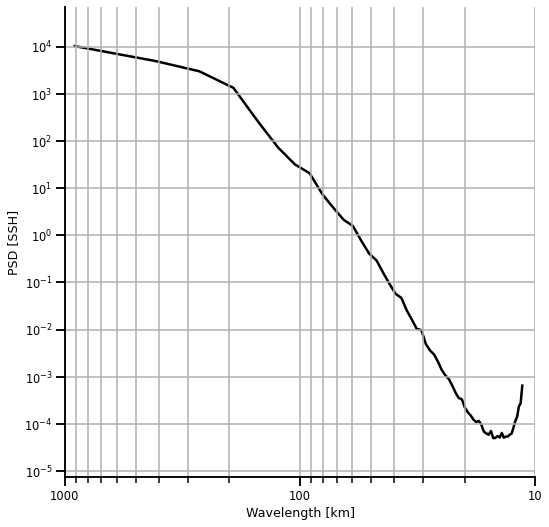
\includegraphics[trim={0 0 0 0},clip, width=3.70cm,height=3.5cm]{00_Oceanbench/content/figures/fourdvarnet_figs/osse_gf_nadir_isotrop.png} &
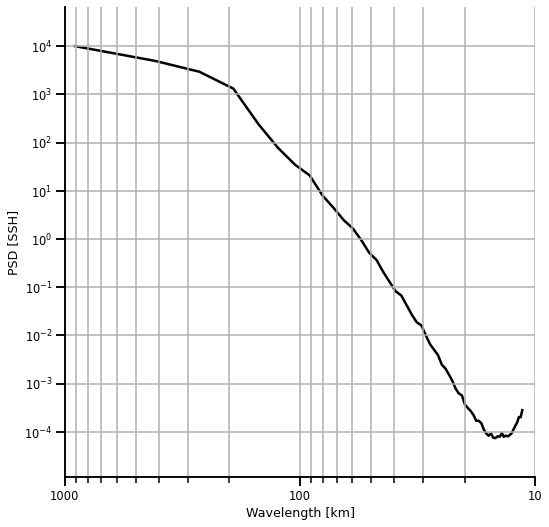
\includegraphics[trim={18mm 0 0 0},clip, width=3.3cm,height=3.5cm]{00_Oceanbench/content/figures/fourdvarnet_figs/osse_gf_nadirswot_isotrop.png} &
\hspace{-5mm}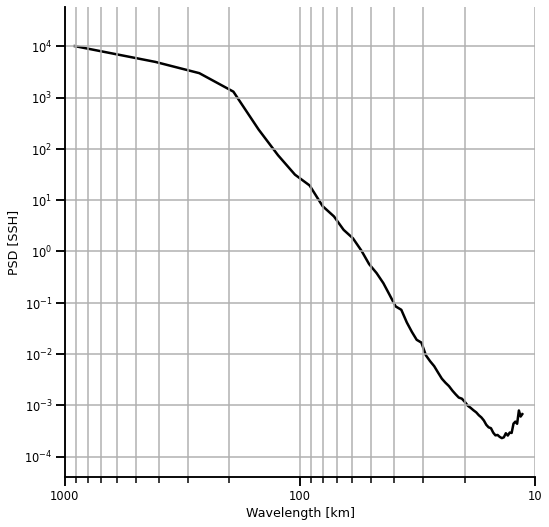
\includegraphics[trim={18mm 0 0 0},clip, width=3.3cm,height=3.5cm]{00_Oceanbench/content/figures/fourdvarnet_figs/osse_gf_nadir_sst_isotrop.png} &
\hspace{-10mm}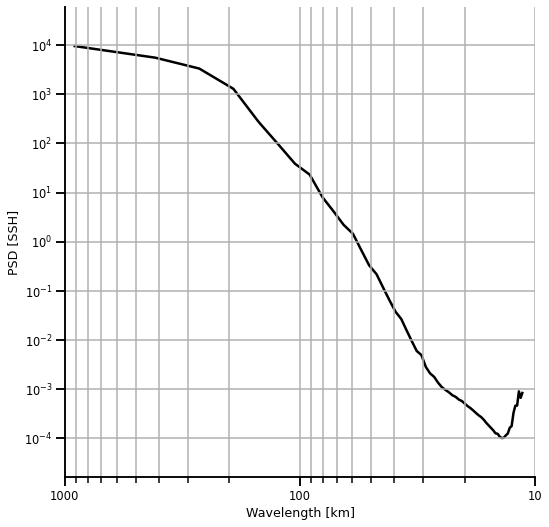
\includegraphics[trim={18mm 0 0 0},clip,width=3.3cm,height=3.5cm]{00_Oceanbench/content/figures/fourdvarnet_figs/ose_gf_isotrop.png} \\
%\vspace{3mm}
%%%%% KINETIC ENERGY %%%%%%%%
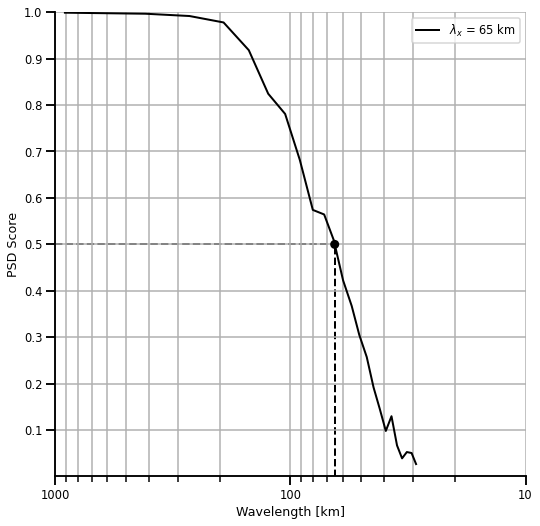
\includegraphics[trim={0 0 0 0}, clip, width=3.70cm,height=3.5cm]{00_Oceanbench/content/figures/fourdvarnet_figs/osse_gf_nadir_1d_psd_score.png} &
\hspace{1mm}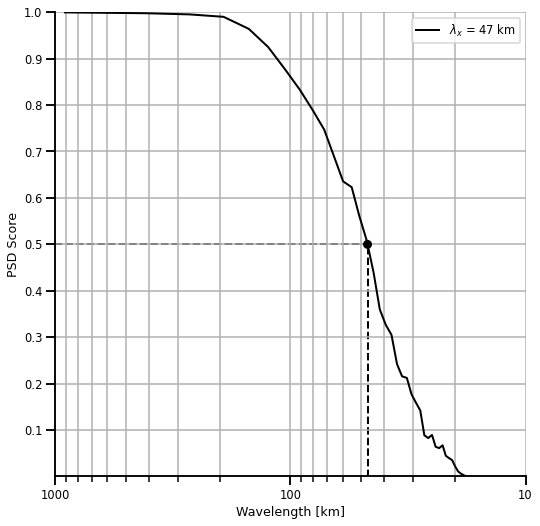
\includegraphics[trim={18mm 0 0 0},clip, width=3.3cm,height=3.5cm]{00_Oceanbench/content/figures/fourdvarnet_figs/osse_gf_nadirswot_1d_psd_score.png} &
\hspace{-4mm}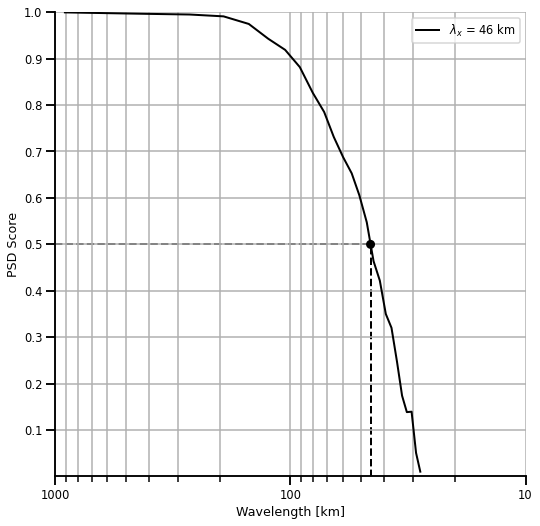
\includegraphics[trim={18mm 0 0 0},clip, width=3.3cm,height=3.5cm]{00_Oceanbench/content/figures/fourdvarnet_figs/osse_gf_nadir_sst_1d_psd_score.png} &
\hspace{-10mm}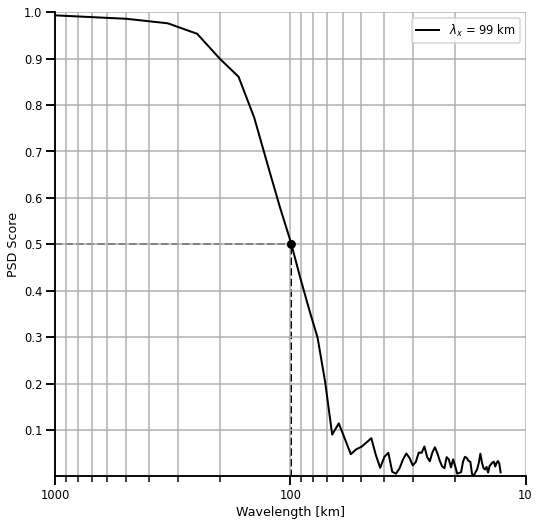
\includegraphics[trim={18mm 0 0 0},clip,width=3.3cm,height=3.5cm]{00_Oceanbench/content/figures/fourdvarnet_figs/ose_gf_1d_psd_score.png} \\
%%%%% RELATIVE VORTICITY %%%%%%%%
\hspace{-4mm}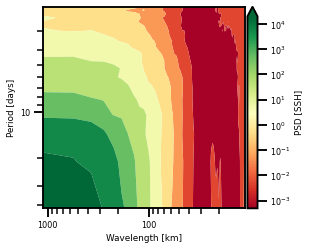
\includegraphics[trim={0 0 23mm 0},clip, width=3.65cm,height=3.5cm]{00_Oceanbench/content/figures/fourdvarnet_figs/osse_gf_nadir_psd_spacetime.png} &
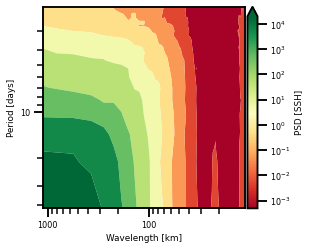
\includegraphics[trim={14mm 0 23mm 0},clip, width=3cm,height=3.5cm]{00_Oceanbench/content/figures/fourdvarnet_figs/osse_gf_nadirswot_psd_spacetime.png} &
\hspace{-5mm}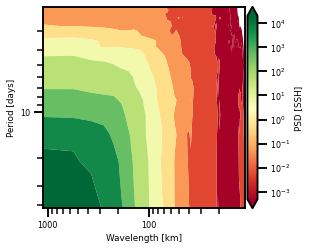
\includegraphics[trim={14mm 0 23mm 0},clip, width=3cm,height=3.5cm]{00_Oceanbench/content/figures/fourdvarnet_figs/osse_gf_nadir_sst_psd_spacetime.png} &
\hspace{-5mm}\includegraphics[trim={14mm 0 0 0},clip,width=3.8cm,height=3.5cm]{00_Oceanbench/content/figures/fourdvarnet_figs/ose_gf_psd_spacetime.png} \\
%%%%% STRAIN %%%%%%%%
\hspace{-4mm}\includegraphics[trim={0 0 23mm 0},clip, width=3.70cm,height=3.5cm]{00_Oceanbench/content/figures/fourdvarnet_figs/osse_gf_nadir_psd_spacetime_score.png} &
\hspace{-2mm}\includegraphics[trim={13mm 0 23mm 0},clip, width=3.1cm,height=3.5cm]{00_Oceanbench/content/figures/fourdvarnet_figs/osse_gf_nadirswot_psd_spacetime_score.png} &
\hspace{1mm}\includegraphics[trim={13mm 0 0 0},clip, width=3.8cm,height=3.5cm]{00_Oceanbench/content/figures/fourdvarnet_figs/osse_gf_nadir_sst_psd_spacetime_score.png} &
 \\
% \vspace{-2mm}
 \hspace{1mm} (a) & \hspace{-5mm} (b) & \hspace{-8mm}(c) & \hspace{-10mm}(d)
\end{tabular}
\vspace{-3mm}
% \caption{Row I - Isotrophic PSD. Row 2 - Isotrophic PSD Score}
\caption{
Power spectrum and associated scores of the 4dVarNet method for each of the four tasks.
The row display in order: (1) the isotropic PSD, (2) the spatial PSD score (using the isotropic PSD for the first three rows and along track PSD for the last row), (3) the space-time PSD, (4) The spacetime PSD score available only in OSSE task.  }

\vspace{-5mm}
\label{fig:oceanbench_psd_4dvarnet}
\end{center}
\end{figure}

% \begin{figure}[h]
% \small
% \begin{center}
% \setlength{\tabcolsep}{1pt}
% \begin{tabular}{cccc}
% \hspace{3mm} NEMO Simulation & 
% \hspace{3mm} MIOST & 
% \hspace{3mm} BFNQG & 
% 4DVarNet \\
% \vspace{-2mm}
% %%%%% SSH %%%%%%%%
% \includegraphics[trim={0 0 38mm 0},clip, width=3.20cm,height=3cm]{content/figures/psd_spacetime/dc20a/nadir4/dc20a_psd_spacetime_nemo_nadir4_ssh.png} &
% \includegraphics[trim={0 0 40mm 0},clip, width=3.2cm,height=3cm]{content/figures/psd_spacetime/dc20a/nadir4/dc20a_psd_spacetime_miost_nadir4_ssh.png} &
% \includegraphics[trim={0 0 38mm 0},clip, width=3.2cm,height=3cm]{content/figures/psd_spacetime/dc20a/nadir4/dc20a_psd_spacetime_bfnqg_nadir4_ssh.png} &
% \includegraphics[width=4.0cm,height=3cm]{content/figures/psd_spacetime/dc20a/nadir4/dc20a_psd_spacetime_4dvarnet_nadir4_ssh.png} \\
% \end{tabular}
% % \vspace{-3mm}
% % \caption{Row I - Isotrophic PSD. Row 2 - Isotrophic PSD Score}
% \caption{The space-time power spectrum decomposition.}
% % \vspace{-5mm}
% \label{fig:appendix_psd_spacetime_NADIR}
% \end{center}
% \end{figure}


% \begin{figure}[h]
% \small
% \begin{center}
% \setlength{\tabcolsep}{1pt}
% \begin{tabular}{cccc}
% \hspace{3mm} DUACS & 
% \hspace{3mm} MIOST & 
% \hspace{3mm} BFNQG & 
% 4DVarNet \\
% % \vspace{-2mm}
% %%%%% SSH %%%%%%%%
% \includegraphics[trim={0 0 38mm 0},clip, width=3.20cm,height=3cm]{content/figures/psd_spacetime/dc20a/nadir4/dc20a_psd_spacetime_score_duacs_nadir4_ssh.png} &
% \includegraphics[trim={0 0 40mm 0},clip, width=3.2cm,height=3cm]{content/figures/psd_spacetime/dc20a/nadir4/dc20a_psd_spacetime_score_miost_nadir4_ssh.png} &
% \includegraphics[trim={0 0 38mm 0},clip, width=3.2cm,height=3cm]{content/figures/psd_spacetime/dc20a/nadir4/dc20a_psd_spacetime_score_bfnqg_nadir4_ssh.png} &
% \includegraphics[width=4.0cm,height=3cm]{content/figures/psd_spacetime/dc20a/nadir4/dc20a_psd_spacetime_score_4dvarnet_nadir4_ssh.png} \\
% \end{tabular}
% % \caption{Row I - Isotrophic PSD. Row 2 - Isotrophic PSD Score}
% \caption{The space-time power spectrum score decomposition.}
% % \vspace{-5mm}
% \label{fig:appendix_psd_score_spacetime_NADIR}
% \end{center}
% \end{figure}
% \newpage
\section{Use Case II: Hydra Recipes} \label{sec:hydra_recipes}

This framework has drastically reduced the overhead for the ML researcher while also enhancing the reprducibility and replicability of the preprocessing steps. In this section we showcase a few examples for how one can use oceanbench in conjunction with hydra to provide recipes for some standard processes.

\subsection{GeoProcessing Recipe}

In this example, we showcase how one can pipe a sequential transformation through the hydra framework. In this example, we open the dataset, validate the coordinates to comply to our standards, select the region of interest, subset the data, regrid the alongtrack data to a uniform grid, and save the data to a netcdf file. See the listing~\ref{hydraconfig:geoprocess} for more information.


\begin{listing}[ht!]
\begin{minted}[frame=lines]{yaml}
# Target Function to initialize
_target_: "oceanbench._src.dataset.pipe"
# netcdf file to be loaded
inp: "${data_directory}/nadir_tracks.nc"
# sequential transformations to be applied
fns:
    # Load Dataset
    - {_target_: "xarray.open_dataset", _partial_: True}
    # Validate LatLonTime Coordinates
    - {_target_: "oceanbench.validate_latlon", _partial_: True}
    - {_target_: "oceanbench.validate_time", _partial_: True}
    # Select Specific Region (Spatial | Temporal)
    - {_target_: "xarray.Dataset.sel", args: ${domain}, _partial_: True}
    # Take Subset of Data
    - {_target_: "oceanbench.subset", num_samples: 1500, _partial_: True}
    # Regridding (AlongTrack -> Uniform Grid)
    - {
        _target_: "oceanbench.regrid", 
        target_grid: ${grid.high_res}, 
        _partial_: True
      }
    # Save Dataset
    - {
        _target_: "xarray.Dataset.to_netcdf", 
        save_name: "demo.nc", 
        _partial_: True
      }
\end{minted}
\label{hydraconfig:geoprocess}
\caption{This is a \texttt{.yaml} which showcases how we can communicate with \texttt{Hydra} framework to list a predefined set of transformations to be \textit{piped} through sequentiall. In this example, we showcase some standard pre-processing strategies to be saved to another netcdf file.}
\end{listing}




\newpage
\subsection{Evaluation Recipe - OSSE}

In this example, we showcase how one can use hydra to do the evaluation procedure. This is the same evaluation procedure that is used to evaluate the effectiveness of the OSSE NADIR experiment. From code snippet~\ref{hydraconfig:geoprocess}, we see that we choose which target function to initialize and we choose the data directory where the \texttt{.netcdf} file is located. Then, we pipe some transformations for the \texttt{.netcdf} file: 1) validate the spatiotemporal coordinates, 2) we select the evaluation region, 3) we regrid it to the target get, 4) we fill in the nans with a Gauss-Seidel procedure, 5) we rescale the coordinates to be in meters and days, and 6) we perform the isotropic power spectrum transformation to get the effective resolution outlined in section~\ref{sec:metrics}.

\begin{listing}[ht!]
\begin{minted}[frame=lines]{yaml}
# Target Function to initialize
_target_: "oceanbench._src.dataset.pipe"
# netcdf file to be loaded
inp: "${data_directory}/ml_result.nc"
# sequential transformations to be applied
fns:
    # Load Dataset
    - {_target_: "xarray.open_dataset", _partial_: True}
    # Validate LatLonTime Coordinates
    - {_target_: "oceanbench.validate_latlon", _partial_: True}
    - {_target_: "oceanbench.validate_time", _partial_: True}
    # Select Specific Region (Spatial | Temporal)
    - {_target_: "xarray.Dataset.sel", args: ${domain}, _partial_: True}
    # Regridding (Uniform Grid -> Uniform Grid)
    - {_target_: "oceanbench.regrid", 
       target_grid: ${grid.reference}, _partial_: True}
    # Fill NANS (around the corners)
    - {_target_: "oceanbench.fill_nans", 
       method: "gauss_seidel", _partial_: True}
    # Coordinate Change (degree -> meters, ns -> days)
    - {_target_: "oceanbench.latlon_deg2m", _partial_: True}
    - {_target_: "oceanbench.time_rescale", 
       freq: 1, unit: "days", _partial_: True}
    # Calculate Isotropic Power Spectrum
    - {_target_: "oceanbench.power_spectrum_isotropic", 
       reference: ${grid.reference}, _partial_: True}
    # Calculate Resolved Spatial Scale
    - {_target_: "oceanbench.resolved_scale", _partial_: True}
    # Save Dataset
    - {_target_: "xarray.Dataset.to_netcdf", 
       save_name: "ml_result_psd.nc", _partial_: True}
\end{minted}
\label{hydraconfig:evaluation}
\caption{This is a \texttt{.yaml} which showcases how we can communicate with \texttt{Hydra} framework to list a predefined set of transformations to be \textit{piped} through sequentiall. In this example, we showcase some standard pre-processing strategies to be saved to another netcdf file.}
\end{listing}





\newpage
\section{Use Case III: XRPatcher}
\label{sec:xrpatcher}

There are many usecases for the \texttt{XRPatcher}. For example, we can do 1D Time chunking, 2D Spatial-Temporal Patches, or 3D Spatial-Temporal Cubes.


\begin{listing}[!ht]
\small
\begin{minted}[frame=lines]{python}
import xarray as xr
import torch
import itertools
from oceanbench import XRPatcher
# Easy Integration with PyTorch Datasets (and DataLoaders)
class XRTorchDataset(torch.utils.data.Dataset):
    def __init__(self, batcher: XRPatcher, item_postpro=None):
        self.batcher = batcher
        self.postpro = item_postpro
    def __getitem__(self, idx: int) -> torch.Tensor:
        item = self.batcher[idx].load().values
        if self.postpro:
            item = self.postpro(item)
        return item
    def reconstruct_from_batches(
            self, batches: list(torch.Tensor), **rec_kws
        ) -> xr.Dataset:
        return self.batcher.reconstruct(
            [*itertools.chain(*batches)], **rec_kws
        )
    def __len__(self) -> int:
        return len(self.batcher)
# load demo dataset
data = xr.tutorial.load_dataset("eraint_uvz")
# Instantiate the patching logic for training
patches = dict(longitude=30, latitude=30)
train_patcher = XRPatcher(
    da=data,
    patches=patches,
    strides=patches,        # No Overlap
    check_full_scan=True    # check no extra dimensions
)
# Instantiate the patching logic for testing
patches = dict(longitude=30, latitude=30)
strides = dict(longitude=5, latitude=5)
test_patcher = XRPatcher(
    da=data,
    patches=patches,
    strides=strides,        # Overlap
    check_full_scan=True    # check no extra dimensions
)
# instantiate PyTorch DataSet
train_ds = XRTorchDataset(train_patcher, item_postpro=TrainingItem._make)
test_ds = XRTorchDataset(test_patcher, item_postpro=TrainingItem._make)
# instantiate PyTorch DataLoader
train_dl = torch.utils.data.DataLoader(train_ds, batch_size=4, shuffle=False)
test_dl = torch.utils.data.DataLoader(test_ds, batch_size=4, shuffle=False)
\end{minted}
\label{listing:xrpatcher}
\caption{\texttt{XRPatcher} integration in Pytorch. We define a PyTorch dataset that handles the \texttt{XRPatcher}. We load an arbitrary dataset with \texttt{xarray}, then we instantiate the \texttt{XRPatcher} with the patching logic, then we instantiate the PyTorch dataset and dataloaders.}
\end{listing}





% \newpage
% \section{Additional Tasks}\label{sec:other_tasks}

In the main paper, we thoroughly outlined the interpolation task to showcase how \texttt{OceanBench} can be used to create automated pipelines for processing and evaluation procedures.
However, there are many other additional tasks that can make use of the \texttt{OceanBench} features. 

\textbf{Denoising}. A simpler problem for interpolation tasks is the denoising problem~\cite{DENOISESURVEY,DENOISESURVEY2}.
The SSH and SST measurements we obtain have inherent noise from the sensors.
A key problem is to calibrate the observations by separating the known noise patterns and the true signal.
There has already been a lot of work from the ML side ranging from amortized predictions~\cite{DENOISESWOT} to end-to-end learning schemes~\cite{DENOISESWOT2}.
Much of this work has been facilitated by the \textit{Ocean-Data-Challenge} group which have a few data challenges related to the denoising problem.
Just like \texttt{OceanBench} was able to create reproducible pipelines from the SSH interpolation challenge listed in section~\ref{sec:data_challenges}, we also believe that one could extend the denoising challenge in the same manner.

\textbf{Forecasting}. This is a special form of extrapolation whereby the temporal domain of the state variable is sufficiently outside of the domain of the observation domain. 
Many previous benchmarking suites already look at forecasting for weather~\cite{weatherbench} and climate~\cite{ClimateBench}.
However, in oceanography, it is also advantageous to do forecasting for problems involving currents~\cite{MLSSC,4DVarNetSSC} and eddies~\cite{OCEANEddyTracking,OKUBO,OKUBOWEISS}.
The \texttt{xrpatcher} will work out of the box for forecasting problems and contributions can be made to \texttt{OceanBench} to include some specific metrics for forecasting as were outlined in~\cite{weatherbench,ClimateBench,ENS10Bench}.

\textbf{Proxy Variables}. There are many other control variables that one could use to improve the interpolation or extrapolation task.
We mentioned SST in section~\ref{sec:data_challenges} because it is the most abundant observations available.
However, there are other important observed variables which could be useful, e.g. Ocean colour, Bigeochemical parameters, and atmospheric variables.
In many other downstream applications, the oceanography community often uses SSH and SST as proxy variables to predict important quantities related to the carbon uptake, e.g. SOCAT~\cite{SOCAT}.
It would be straightforward to include a specific variable (and the associated preprocessing operations) into \texttt{OceanBench}.

\textbf{Dimension Reduction}. We often have very resolution spatiotemporal fields.
which poses a very big challenge for learning due to the high correlations exhibited by spatiotemporal data and high dimensionality.
A workaround for this is to learn a latent representation which retains as much relevant information as possible for the given task.
In the ocean sciences, this is known as \textit{Reduced Order Modeling} (ROM) or more generally dimensionality reduction which has been frequently used for adaptive meshes for physical models~\cite{NEMOEOF}.
This could be used for pretraining fields to latent embeddings which could be useful for downstream tasks like anomaly detection~\cite{SSTFLOWANOMALY}.
% In modern diffusion models, most of the operations are within the latent domain without any loss of quality in the generative results.


\textbf{Surrogate Modeling}. 
Physical model simulations are very expensive and ML has played a role in learning surrogate models to descrease the computational intensity~\cite{ML4OCN,MLCLOSURE}.
We have a decently long spatiotemporal field over a region of interest which could be used to learn a surrogate model to mimic the dynamics of that region.
This is also very useful for hybrid schemes whereby we have parameterizations to account for processes that are missing from low resolution simulations.~\cite{MLOCNPARAMETERIZATION,MLOCNPARAMETERIZATION2, MLOCNPARAMETERIZATION3, MLOCNPARAMETERIZATION4}.



% \subsection{Main Tasks}

% \subsubsection{Interpolation/Extrapolation}

% The two main tasks we can define from this problem setup are: 1) interpolation/extrapolation and 2) forecasting (which can be seen as extrapolation in Time). 
% Both interpolation and extrapolation are when the domain for the $\mathcal{T}$ always falls between the past and the present, i.e., $\mathcal{T}\in[0, T]$ where $T$ is the current Time. 
% We define interpolation as the case where the observations along the boundary of the domain are equal to the boundary of the desired reconstruction domain, i.e., $\partial\boldsymbol{\Omega}_{obs} = \partial\boldsymbol{\Omega}_g$, and extrapolation as the case where the boundary of the observation domain lies entirely inside of the boundary of the reconstructed domain, i.e., $\partial\boldsymbol{\Omega}_{obs} \subset \partial\boldsymbol{\Omega}_g$. 
% Forecasting refers to the problem when the temporal domain $\mathcal{T}$ lies outside of the present, i.e., $T+\tau$ where $\tau$ is some step within the future that is outside of the temporal observation domain, $\mathcal{T}\in[0, T]$. 
% Note that this is irrespective of the spatial domain or its boundaries. 
% In the rest of this paper, we will look exclusively at the interpolation problem, but we refer to the reader to section~\ref{sec:other_tasks} in the appendix for a more detailed look at the other tasks.

% \begin{equation}
%     \mathbf{y} = \mathcal{H}(\mathbf{x})
% \end{equation}


% where $\mathbf{y}\in\boldsymbol{\Omega_p}$ is the incomplete observation within some subdomain and $\mathbf{x}\in\boldsymbol{\Omega}$  is the true observation over the full domain.



% \subsubsection{Forecasting}

% \begin{equation}
%     \boldsymbol{u}_{t+\delta t} = \mathcal{M}(\boldsymbol{u}(\mathbf{x}, t+\delta t), \delta t; \boldsymbol{\theta})
% \end{equation}

% \subsection{SubTasks}

% \subsubsection{Surrogate/Hybrid/Parameterizations}

% \begin{equation}
%     \frac{\partial u}{\partial t} = \mathcal{M}(\boldsymbol{u}(\mathbf{x},t), \mathbf{x}, t; \theta)
% \end{equation}





% \newpage
% \section{Machine Learning Method Ontology} \label{sec:ml_ontology}

Although this paper does not focus on the explicit methods used for SSH interpolation, we would like to give a readers a brief overview of some of the most popular methods in the literature.

\subsection{Coordinate-Based methods}

These methods learn a direct mapping between the coordinate vectors to the scalar or vector values. 
%
\begin{align}
    \boldsymbol{y}_{obs} &= \boldsymbol{f}(\mathbf{x},t;\boldsymbol{\theta})+\boldsymbol{\epsilon}(\mathbf{x},t)
\end{align}
%
This is better known as \textit{functa}~\cite{FUNCTA} which parameterizes the field directly as a model.

\textbf{Functional}. Optimal Interpolation (OI) is the most common method used for many of the operational methods~\cite{DUACS}. It is a non-parametric, functional method which is built upon covariance and precision matrices. In the machine learning community, these methods are known as Gaussian Process~\cite{GPsBIGDATA} and in the geostatistics community, this is known as Kriging~\cite{KRIGINGREVIEW}.

\textbf{Basis Function}. This is an easy simplification to the functional by introducing parametric basis functions. In particular, the MIOST~\cite{MIOST} algorithm will be adopted in the new operational products for SSH interpolation. It is a custom basis function based on Wavelet analysis which is scale-aware and scalable.

\textbf{Neural Fields}. Neural fields (NerFs) are a very popular set of methods that use neural networks to effectively learn the basis function through a composition of weights, biases and activations~\cite{NERFSSSH}.
Furthermore, one can add physics-informed constraints to the loss function which mirror that of a PDE~\cite{PINNS}.
In many cases, especially with many auxillary inputs, we don't have access the PDE so one fit a NN directly to the observations with a fully connected neural network~\cite{SOCAT}.


\subsection{Grid-Based Methods}

In practice, we often consider the field at a specific discretized setting like a uniform grid or mesh. 
This is because we typically operate on and store these fields as multi-dimensional arrays which are only defined on a subspace of the entire continuous domain. 
We denote a discretized spatial representation as $\boldsymbol{\Omega}_g\subset\mathbb{R}^{N_s}$. 
We can simplify this notation by including the domain within the operator. So equation~\ref{eq:interp_problem} like so:
\begin{equation}\label{eq:interp_problem_discretized}
    \boldsymbol{\eta}(\boldsymbol{\Omega}_{obs},t ) = \mathcal{H}\left(\boldsymbol{\eta}(\boldsymbol{\Omega}_g,t), t, \boldsymbol{\mu},  \boldsymbol{\varepsilon} \right) 
    % + \boldsymbol{\varepsilon}(\boldsymbol{\Omega}_g, t)
\end{equation} 
%
In this equation, $\mathcal{H}$ is the observation operator that transforms the field from the full discretized domain, $\boldsymbol{\Omega}_g$, to the observation domain, $\boldsymbol{\Omega}_{obs}\subset\mathbb{R}^{N_{obs}}$.

\textbf{Direct Methods}. 
These methods take the noisy, incomplete observations and directly feed it to a model that returns the full reconstructed field.
They typically involve training a convolutional neural network or recurrent neural network on pairs of corrupted observations to learn the reconstruction~\cite{SuperResSurvey,IMAGE2IMAGETRANSLATION, IMAGE2IMAGETRANSLATION2}.
This has seem some sucess in applications related to SSH interpolation~\cite{SSHInterpUNet,SSHInterpConvLSTM, SSHInterpAttention}.

\textbf{Traditional Data Assimilation.}
There are many traditional methods that are rooted in data assimilation~\cite{DAGEOSCIENCE}.
For example, the GLORYS~\cite{GLORYS12} method propagates the physical model forwards in time and then \textit{updates} the state based on observations periodically.
A simpler approach is to use a nudging scheme coupled with a simpler physical model~\cite{BFNQG}.


\textbf{End-to-End Learning}. These methods try to solve the problem by learning and end-to-end scheme to solve the model inversion problem.
This is very similar to implicit methods that define a cost function to minimize instead of a minimizing the parameters of a prior model.
Plug-in-Play priors are a popular class of methods that pre-train priors on auxillary observations and then use the prior in the inversion scheme~\cite{DEEPUNFOLDING}.
This has seen a lot of success in SSH interpolation~\cite{4DVARNETSWOT,4DVARNETSST,4DVarNetSSC}.



% \newpage
% In practice, we only consider the field at a specific discretized setting like a uniform grid or mesh. 
% This is because we typically operate on and store these fields as multi-dimensional arrays which are only defined on a subspace of the entire continuous domain. We denote this discretized spatial representation as $\boldsymbol{\Omega}_g\subset\mathbb{R}^{N_s}$. We can simplify this notation by including the domain within the operator, like so:
% %
% \begin{equation} \label{eq:ssh_field_discretized}
%     \eta =\boldsymbol{\eta}(\boldsymbol{\Omega}_g,t),
% \end{equation}
% %
% This is more reflective of how we use operators in practice as we typically insert the field as a grid or multi-dimensional spatial array through a series of mathematical operations.
% We can further discretized this field through the time domain whereby we have a finite set of observations in time, $D_t$. Let's say that we have $N_t$ ordered samples in time between a defined interval of $[0,T]$, i.e. $\mathcal{T}=\left\{ t_t \in [0,T]\right\}_i^{N_{t}}$. In some settings, this could be a uniform observation that is hourly for the period of 1 day, i.e. $N_t=24$, or daily over the period of 10 years, i.e. $N_t=3650$. In more realistic settings, this could be an irregular pattern.
% Equation~\eqref{eq:ssh_field_discretized} assumes the full field is observed. In practice, we observe a corrupted, incomplete version of this SSH field s.t.
% %
% \begin{equation}\label{eq:obs_operator_discretized}
%     \boldsymbol{\eta}(\boldsymbol{\Omega}_{obs},t ) = \mathcal{H}\left(\boldsymbol{\eta}(\boldsymbol{\Omega}_g,t), t, \boldsymbol{\mu},  \boldsymbol{\varepsilon} \right) 
%     % + \boldsymbol{\varepsilon}(\boldsymbol{\Omega}_g, t)
% \end{equation} 

% In this equation, $\mathcal{H}$ is the observation operator that transforms the field from the full discretized domain, $\boldsymbol{\Omega}_g$, to the observation domain, $\boldsymbol{\Omega}_{obs}\subset\mathbb{R}^{N_{obs}}$. 
% The observation domain, $\boldsymbol{\Omega}_{obs}$, are the spatial coordinates, $\mathbf{x}$, where the SSH has been observed which is a proper subset of the full domain, i.e. $\boldsymbol{\Omega}_{obs}\subseteq\boldsymbol{\Omega}_g$.

% \begin{align} \label{eq:interp_problem}
%     \mathcal{M}_{\boldsymbol{\theta}} &: \boldsymbol{\eta}_{obs}(\mathbf{x}, t, \boldsymbol{\mu}) \rightarrow \boldsymbol{\eta}(\mathbf{x},t) \hspace{10mm}
%      \boldsymbol{\Omega}_{obs} \in \mathbb{R}^{N_{obs}} \hspace{5mm} 
%     \boldsymbol{\Omega}_g \in \mathbb{R}^{N_s} \hspace{5mm} 
%     t \in \mathcal{T}.
% \end{align}


% \subsubsection{Hybrid Schemes} \label{sec:bfn}

% This includes Backwards-Forwards Nudging with a simpler model like the Quasi-Geostrophic equations.

% \subsubsection{Direct Methods}

% These feature methods that directly take in the sparse SSH fields with \tocite{Recent Papers}

% \subsubsection{Data Assimilation}

% \begin{align}
%     \boldsymbol{\theta}^* &= \underset{\boldsymbol{\theta}}{\text{argmin}} \hspace{2mm} \mathcal{L}(\mathbf{x}_{gt}, \mathbf{x}(\boldsymbol{\theta})) \\
%     \mathbf{x}^*(\boldsymbol{\theta}) &= \underset{ \mathbf{x}^*}{\text{argmin}}  \hspace{2mm} \mathcal{U}\left(\mathbf{x}(\boldsymbol{\theta}) \right)
% \end{align}

% where $\mathcal{L}$ is some loss function to find the best parameters and $\mathcal{U}$ is some energy function to minimize the state.

% \subsubsection{End-to-End 4DVariational Methods} \label{sec:4dvarnet}

% These methods take a variational approach whereby we directly define the cost function we wish to solve \tocite{Ronan}. To speed up the convergence of these methods, a meta-learning based method was introduced to learn the gradient descent\tocite{Ronan}. In addition, this has been improved with the addition of sea surface temperature as an additional term in the cost function. 



% \newpage
% \section{Target Audience}
% \subsection{Project Vision}
While this tool is general in scope, we specifically target three audiences: 1) the domain expert who may want to use and understand and investigate SSH in relation to other important EO quantities, 2) machine learning researchers who may want to investigate how to make a better model for SSH interpolation, and 3) downstream users who are interested in adopting some techniques for their own domain-specific applications that may rely on SSH like tracking ocean currents~\tocite{}, investigating biogeochemical transport~\tocite{}, or global climate change~\tocite{}. In the following subsections, we give a more detailed description about the users and how might they benefit from \texttt{OceanBench}.

\textbf{Domain Experts}. We consider \textit{domain experts} who are experts in different domains of oceanography. ...


\textbf{ML Researchers}. We consider those who are expert ML researchers but may lack...



\textbf{Down Stream Users}. We also envision a broader adoption of the framework across research labs interested in having standardized data challenges for their own research purposes. There are independent groups choosing datasets for their specific use cases however, this framework can serve as an easy way to integrate their existing methodologies into the set of common tools to be used and improved by multiple communities. By establishing a relatively consistent problem set, we hope that any innovation can be easily understood and transferred across domains.
% \newpage
% \section{Limitations} \label{sec:appendix_limitations}

\subsection{Framework Limitations}

While we have advertised \texttt{OceanBench} as a unifying framework that provides standardized processing steps that comply with domain-expert standards, we also highlight some potential limitations that could hinder its adoption for the wider community.

\textbf{Data Serving}. We provide a few datasets but we omit some of the original simulations. We found that the original simulations are terabytes/petabytes of data which becomes infeasible for most modest users (even with adequate CPU resources).  
This is very big problem and if we want to have a bigger impact, we may need to do more close collaborations with specified platforms like the Marine Data Store~\citep{MDSOCEANPHYSICS,MDSBIOGEOCHEMICAL,MDSOCEANPHYSICSENS,MDSINSITU,MDSWAVES,MDSALONGTRACK,MDSSSH} or the Climate Data Store~\citep{CDSREANALYSISSST,CDSOBSSST,CDSOBSOC,CDSOBSSSTENS}. Furthermore, there are many people that will not be able to do a lot of heavy duty research which indirectly favours institutions with adequate resources and marginalizing others. 
This is also problematic as those communities tend to be the ones who need the most support from the products of such frameworks.
We hope that leaving this open-source at least ensure that the knowledge is public.

\textbf{Framework Dependence}. The user has to "buy-into" the \texttt{hydra} framework to really take advantage of \texttt{OceanBench}. This adds a layer of abstraction and a new tool to learn. 
However, we designed the project so that high level usage does not require in-depth knowledge of the framework. 
In addition, we hope that, despite the complexity of project, users will appreciate the flexibility and extensibility of this framework.


\textbf{Lack of Metrics}. We do not provide the most exhaustive list of metrics available with the ocean community. In fact, we also believe that many of these metrics are often poor and do not effectively assess the goodness of our reconstructions. 
However, we do provide a platform that will hopefully be useful and easy to implement new and improved metrics.
Furthermore, having a wide range of metrics that are trusted across communities may help to improve the overall assessment of the different model performances~\cite{METRICSAVERAGE}.

\textbf{Limited ML Scope}. 
The framework does not support nor promote any machine learning methods and we lack any indication of comparing ML training and inference performance. 
However, we argue that a benchmark framework will allow us to effectively compare whichever ML methods are demonstratively the best which is a necessary preliminary step which offers users more flexibility in the long-run.

\textbf{Broad Oceans Application Scope}. 
We have targeted a broad ocean-application scope of state estimation.
However, there may be more urgent applications such as maritime monitoring, object tracking, and general ocean health.
However, we feel that many downstream applications require high-quality maps.
In addition, those downstream applications tend to be very complicated and are not always straightforward to apply ML under those instances.

\textbf{Full Pipeline Transparency}. We use a lot of different \texttt{xarray}-specific packages which have different design principles, assumptions and implementations. This may give the users an illusion of simplicity and transparency to real-world use. However, there are many underlying assumptions within each of the packages that may occlude a lot of design decisions.
Despite this limitation, we believe that being transparent about the processing steps and being consistent with the evaluation procedure will be beneficial for the ML research community.

\textbf{Scalability}. Scaling this to many terabytes or petabytes of data is easily the biggest limitation of the framework. In addition, we have only showcased demonstrations for 2D+T fields which are much less expensive than 3D+T fields.

\textbf{Deployability}. MLOPs has many wheels and it is not easy to integrate into existing systems. We offer no solutions to this. 
However, we believe that our framework is fully transparent in the assumptions and use cases which will facilitate some adoption into operational systems where they can further modify it for their use cases (see the evolution of \texttt{WeatherBench} and \texttt{ClimateBench}).

\textbf{Visualization Tools}.
We do not incorporate a high quality visualization tool that allows users to do pre- and post-analysis at a large scale. 
We do provide some simple visualization steps that are ML-relevant (see the GitHub repo) but it is very limited to ML standards.
One solution is to interface our pipeline with the source of many ocean datasets, e.g. Climate Data Store~\citep{CDSREANALYSISSST} or Marine Data Store~\citep{MDSOCEANPHYSICS}, then we can offset this task to them where they can offer better quality visualization tools.

\newpage
\subsection{Data Challenge Limitations}

We have showcased the SSH interpolation edition as a data challenge which could be helpful for real applications. 
However, in section~\ref{sec:problem_scope} we alluded to the greater task of general ocean state estimation which is more pertinent to the ocean sciences yet we don't address this directly with our data challenges.
Furthermore, we claim that the data challenges presented will help the ocean community with using ML for SSH interpolation.
Below, we outline some limitations which address these criticisms.

\textbf{Not the overall objective}. 
We recognized that we are far away from the actual reanalysis and forecasting goals of full state estimation. 
However, we argue that that is a rather ambitious challenge which will require a lot of interdisciplinary work across communities. 
In the meantime while we work towards that goal, operational centers could possibly improve their current products from ML-based techniques would would benefit downstream applications that deal directly with SSH.
Furthermore, SSH is an important variable in describing the full ocean state.
So a robust set of techniques that are able to solve the interpolation tasks could (in principal) be used to solve extra tasks.

\textbf{Small Region \& Period}.
We only feature a small region and period over the Gulfstream which is not representative of the different global regimes. 
This also does not take into account real things like \textit{data drift} which will inevitable occur in operational settings.
However, this is a dynamical regime and a well-studied area which does have some importance for specific communities and the results obtained offer some transferability to other dynamical regimes.
In addition, this area will have good coverage due to the new SWOT mission~\cite{SWOT} which will allow for further validation in the future.
Lastly, the area is small enough where the beginning stages for ML researchers is not overwhelmed with problems involving scale (even though we eventually want to arrive at global schemes).
We hope to extend our challenges to more relevant scenarios~\cite{MDSALONGTRACK}.

\textbf{Simulations versus Reanalysis}. We use simulations for the OSSE experiments instead of reanalysis. This is an open research question as it is unclear whether it's better to pretrain models on simulated ocean data or reanalysis ocean data. In future updates, we plan to add the reanalysis data to extend the challenge.

\textbf{Efficacy of OSSE Experiments}. We alluded to the idea that the OSSE experiments may not reflect the overarching goal of the user yet we provide more OSSE experiments than OSE experiments.
We acknowledged that it often does not coincide exactly with the OSE experiments which may give users a false sense of accomplishment and immediate transferability. 
However, we try to provide a framework where one could thoroughly experiment with the learning problem on OSSE configurations which can facilitate transfer learning to other domain-specific tasks.
We also anticipate that new \textit{real} SWOT data~\cite{SWOT} will start to become more available which will allow us to design better, realistic OSE experiments.

\textbf{Noise Characterization}.
Real data has noise to content with and we do not account for that within the SSH interpolation experiments.
The true noise we see in operational settings is structured and this would require more knowledge outside the scope of our teams expertise.
A more improved challenge would take these considerations into account.
We leave this as a future challenge for the community and we hope our platform can help facilitate this.

\textbf{Uncertainty Quantitification}.
We prefaced the problem statement with the idea of data assimilation which is the notion of \textit{state/parameter estimation under uncertain conditions and incomplete information}~\citep{DAGEOSCIENCE}.
However, we have not addressed any notion of uncertainty at all throughout the paper.
Uncertainty is difficult to quantify and we don't want to impose too many restrictions until we more sure about the efficacy of ML for easier problems.
However, to move the problem setting towards a more realistic setting, we can start to introduce metrics and additional requirements from future challenges, e.g. mean and standard deviation estimates or ensemble predictions.


\textbf{Operational Constraints}.
The real use case of SSH interpolation will involve global data and/or high-resolution data. 
This involves dealing with very high-dimensional spatiotemporal global state-space.
In practice, the necessity for the scalability of the method is of paramount importance.
However, there are also areas within the ML research community who are looking into many ways we can scale up physical models~\citep{VEROS,OCEANANIGANS} and machine learn models for geoscience tasks~\citep{SFNO}.
We anticipate that once a set of solutions are excepted by a community, the scalability will come later.




% \newpage
% \subsection{Dataset Limitations}



% \textbf{Limitations}. The scope of this is very specific to researchers who are interested in ML. It only serves as a baseline design. If one would like to scale, it would require much more engineering work to get everything to connect. This is already seen if we are to load datasets of PBs. In addition, this requires researchers to have access to considerably large machines to be able to run their own preprocessing schemes. We do our best to provide toy datasets of a modest size however, inevitably, one will probably need to work with larger and large datasets.

% \subsection*{Broader Impact}
% \label{sec:impact}

% The theme of interpolation is present in many applied communities with different names, e.g. kriging in ecology/hydrology, Optimal interpolation in oceanography, and Gaussian processes in statistics. We hope that this work bridges this gap between the communities and we invite other works to try to highlight concrete ways that machine learning and classic physics have commonalities.

% In the oceanography community in particular, we especially hope to see more adoption of machine learning methods for interpolation. DUACS is ultimately a closed-system so the wider scientific community does not have access to the algorithm. Our OI baseline hopefully unveils some of the finer details of the method. However, in general, the standard OI methods used in the applied community cannot keep up with the massive influxes of observations we receive. So this work is a first step in demonstrating that neural networks (in particular NerFs) are a viable, simpler, and scalable alternative.
% \section*{User Guide}
% \addcontentsline{toc}{section}{User Guide}

% \addcontentsline{toc}{section}{Bibliography}
  % \putbib[00_Oceanbench/content/bibliographies/full.bib]
\end{bibunit}


\clearemptydoublepage
% Pour avoir la quatrième de couverture sur une page paire
% To have the back cover on an even page
\cleartoevenpage[\thispagestyle{empty}]
\markboth{}{}
% Plus petite marge du bas pour la quatrième de couverture
% Shorter bottom margin for the back cover
\newgeometry{inner=30mm,outer=20mm,top=40mm,bottom=20mm}

%insertion de l'image de fond du dos (resume)
%background image for resume (back)
\backcoverheader

% Switch font style to back cover style
\selectfontbackcover{ % Font style change is limited to this page using braces, just in case

\titleFR{titre (en fran\c cais)..............}

\keywordsFR{de 3 \`{a} 6 mots clefs}

\abstractFR{Eius populus ab incunabulis primis ad usque pueritiae tempus extremum, quod annis circumcluditur fere trecentis, circummurana pertulit bella, deinde aetatem ingressus adultam post multiplices bellorum aerumnas Alpes transcendit et fretum, in iuvenem erectus et virum ex omni plaga quam orbis ambit inmensus, reportavit laureas et triumphos, iamque vergens in senium et nomine solo aliquotiens vincens ad tranquilliora vitae discessit.
Hoc inmaturo interitu ipse quoque sui pertaesus excessit e vita aetatis nono anno atque vicensimo cum quadriennio imperasset. natus apud Tuscos in Massa Veternensi, patre Constantio Constantini fratre imperatoris, matreque Galla.
Thalassius vero ea tempestate praefectus praetorio praesens ipse quoque adrogantis ingenii, considerans incitationem eius ad multorum augeri discrimina, non maturitate vel consiliis mitigabat, ut aliquotiens celsae potestates iras principum molliverunt, sed adversando iurgandoque cum parum congrueret, eum ad rabiem potius evibrabat, Augustum actus eius exaggerando creberrime
docens, idque, incertum qua mente, ne lateret adfectans. quibus mox Caesar acrius efferatus, velut contumaciae quoddam vexillum altius erigens, sine respectu salutis alienae vel suae ad vertenda opposita instar rapidi fluminis irrevocabili impetu ferebatur.
Hae duae provinciae bello quondam piratico catervis mixtae praedonum.}



\titleEN{titre (en anglais)..............}

\keywordsEN{de 3 \`{a} 6 mots clefs}

\abstractEN{Eius populus ab incunabulis primis ad usque pueritiae tempus extremum, quod annis circumcluditur fere trecentis, circummurana pertulit bella, deinde aetatem ingressus adultam post multiplices bellorum aerumnas Alpes transcendit et fretum, in iuvenem erectus et virum ex omni plaga quam orbis ambit inmensus, reportavit laureas et triumphos, iamque vergens in senium et nomine solo aliquotiens vincens ad tranquilliora vitae discessit.
Hoc inmaturo interitu ipse quoque sui pertaesus excessit e vita aetatis nono anno atque vicensimo cum quadriennio imperasset. natus apud Tuscos in Massa Veternensi, patre Constantio Constantini fratre imperatoris, matreque Galla.
Thalassius vero ea tempestate praefectus praetorio praesens ipse quoque adrogantis ingenii, considerans incitationem eius ad multorum augeri discrimina, non maturitate vel consiliis mitigabat, ut aliquotiens celsae potestates iras principum molliverunt, sed adversando iurgandoque cum parum congrueret, eum ad rabiem potius evibrabat, Augustum actus eius exaggerando creberrime
docens, idque, incertum qua mente, ne lateret adfectans. quibus mox Caesar acrius efferatus, velut contumaciae quoddam vexillum altius erigens, sine respectu salutis alienae vel suae ad vertenda opposita instar rapidi fluminis irrevocabili impetu ferebatur.
Hae duae provinciae bello quondam piratico catervis mixtae praedonum.}

}

% Rétablit les marges d'origines
% Restore original margin settings
\restoregeometry

\end{document}
